\documentclass[phd,tocprelim]{cornell}
%
% tocprelim option must be included to put the roman numeral pages in the
% table of contents
%
% The cornellheadings option will make headings completely consistent with
% guidelines.
%
% This sample document was originally provided by Blake Jacquot, and
% fixed up by Andrew Myers.
%
%Some possible packages to include
\usepackage{graphicx,pstricks}
\usepackage{graphics}
\usepackage{moreverb}
\usepackage{subfigure}
\usepackage{epsfig}
\usepackage{subfigure}
\usepackage{hangcaption}
\usepackage{txfonts}
\usepackage{palatino}


\usepackage{alltt}

\usepackage{algorithm}
\usepackage{multicol}
\usepackage{bbold}

\usepackage{pstricks-add}

\usepackage{algorithmic}
%\usepackage{amsmath}


%if you're having problems with overfull boxes, you may need to increase
%the tolerance to 9999
\tolerance=9999

\bibliographystyle{plain}
%\bibliographystyle{IEEEbib}

\renewcommand{\algorithmicrequire}{\textbf{Input:}}
\newtheorem{theorem}{Theorem}[section]

\newtheorem{definition}{Definition}
\newtheorem{lemma}[definition]{Lemma}
\newtheorem{corollary}[definition]{Corollary}

\renewcommand{\caption}[1]{\singlespacing\hangcaption{#1}\normalspacing}
\renewcommand{\topfraction}{0.85}
\renewcommand{\textfraction}{0.1}
\renewcommand{\floatpagefraction}{0.75}

\title {Community Detection in Large Networks}
\author {June Andrews}
\conferraldate {May}{2012}
\degreefield {Ph.D.}
\copyrightholder{June Andrews}
\copyrightyear{2012}

\begin{document}

\maketitle
\makecopyright


\begin{abstract}

Graphs are used to represent various large and complex networks in scientific applications.  In order to understand the structure of these graphs, it is useful to treat a set of nodes with similar characteristics as one community and analyze the community's behavior as a whole.  Finding all such communities within the graph is the object of community detection.  In our research, we compare dozens of existing community detection methods and develop a new class of algorithms for finding communities.

\end{abstract}

\begin{biosketch}
June Andrews was born in San Diego, 1985.
She attended University of California, Berkeley for her undergraduate degree in Electrical Engineering and Computer Science, with a minor in Applied Mathematics.
She is now completeing her doctoral degree in Applied Mathematics at Cornell University.
\end{biosketch}

\begin{dedication}
\begin{figure}[!h]
\centering

\includegraphics[width=3in]{Figures/windy}
\caption{\it Phil Andrews 1955 - 2011}
\end{figure}

Here's to you Da.
\end{dedication}

\begin{acknowledgements}
It goes without saying, these people have been inspiring forces of nature to work with:
\begin{itemize}
\item Len Kulbacki
\item Coach Wilson
\item James Sethian
\item Patricia Kovatch
\item John Hopcroft
\item Steve Strogatz
\item Jon Kleinberg
\end{itemize}
\end{acknowledgements}

\contentspage
\tablelistpage
\figurelistpage

\normalspacing \setcounter{page}{1} \pagenumbering{arabic}
\pagestyle{cornell} \addtolength{\parskip}{0.5\baselineskip}

\chapter{Introduction}

\section{Community Detection}

\begin{figure}[!b]
\centering
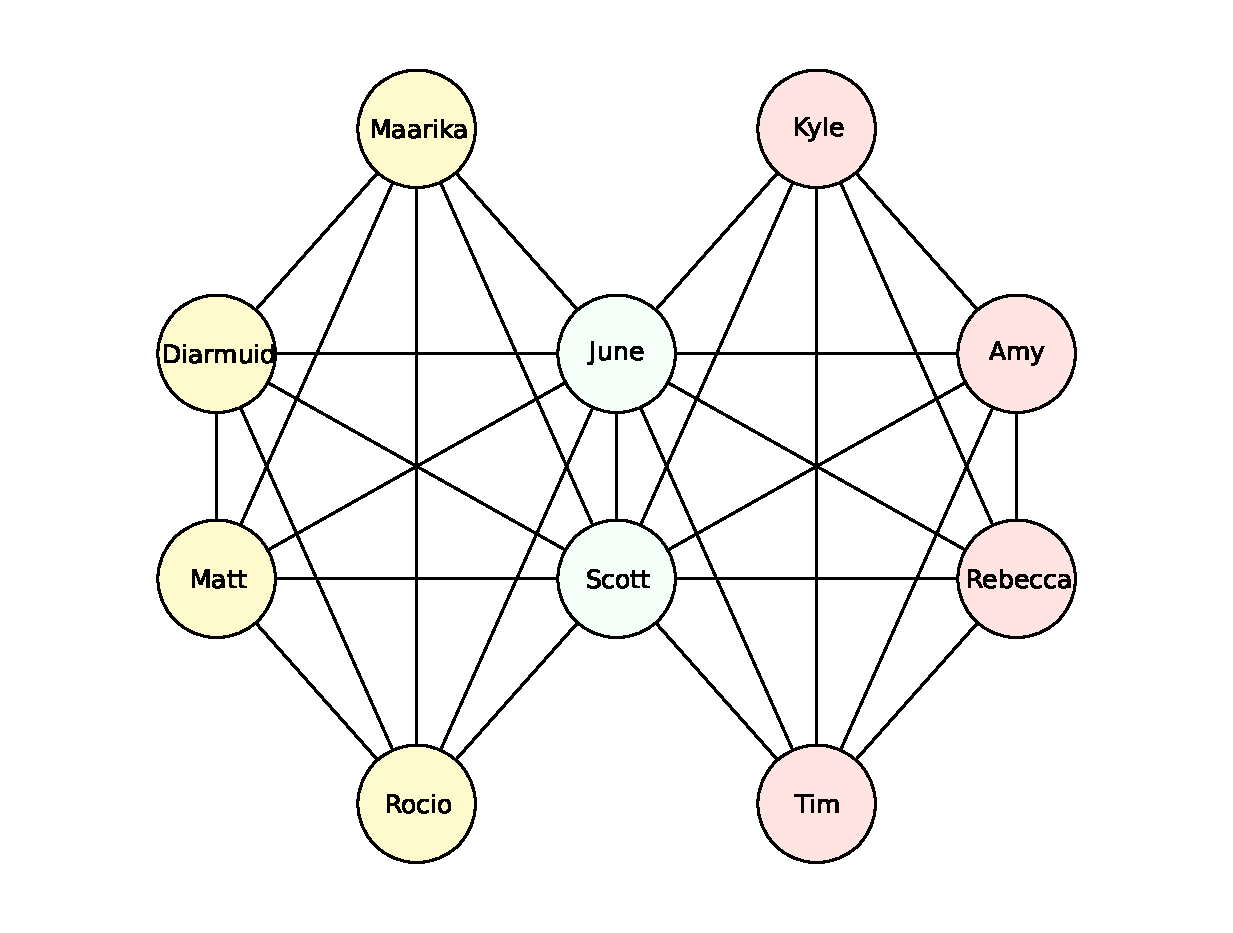
\includegraphics[width=3in]{Figures/visually_simple}
\caption{A simple graph of people and their friendships.  The graph is regular enough to reveal two communities.}
\label{fig_simple}
\end{figure}

Consider an application that studies objects and the interactions between those objects.  The application could study anything from people and their friendships, to papers and their citations; a variety of applications fall into this format.  If we let nodes represent the objects and edges represent the interactions between those objects, we can store the application's data in a graph.  While it can be possible for the application to draw conclusions by looking at every node within the graph, if the graph is large and complex, analyzing every node can be unmanageable and can produce incomprehensible results.   We simplify the graph by finding communities of nodes.  In particular, we want communities, whose members interact with each other in a particular way and interact with non-members of the community in a different way. If such a community is found, then two questions arise.  How are members of the community related?  How does the community interact with the rest of the graph?  Given answers to these questions, we can comprehend what is happening in the graph at a local level.  For social networks, we know that communities exist \cite{JTODO}.  Due to the large, complex nature of social networks, communities can be hard to find.  In order to find communities, we must develop the ability to see the forest through the trees.  We have to be able to extract the communities of nodes from the interactions of the graph.  This is the object of community detection.


Given a graph, there are two prominant questions community detection seeks to answer.  The first, what is a community and the second, what are the communities?  Several approaches have been developed to answer these two questions, some with a particular application as motivation.  We outline the coupling of a few sciences and one of their preferred detection methods in Table \ref{tbl_app_method}. Prior to $2002$, most development of community detection was done within the fields of the applications.  Since then, computer scientists have contributed a large volume of advances towards answering these two questions for applications in general.  The first goal of this thesis to try and tie together a portion of these advances into a cohesive understanding of community detection.  The second is to use our perspective to create fast and parallel algorithms.

\begin{table}[!h]
\centering
\begin{tabular}{l|l}
Application & Community Detection Method \\ \hline
Parallel Computation Distribution & $k-$means clustering \cite{JTODO} \\
Physics & Belief Propogation \cite{JTODO}\\
Search Queries & \cite{JTODO} \\
Sociology & \cite{JTODO} \\
Storage of Large Matrices & Spectral Analysis \cite{JTODO} \\
Taxonomy & Neighbor Joining \cite{JTODO} \\
\end{tabular}
\caption{A subset of applications and one of their preferred community detection methods.}
\label{tbl_app_method}
\end{table}


\section{Graph Partitioning Methods}

For many applications the object is to partition the graph into disjoint components.  We call each component a community.  There are an exponential number of possible partitions, but not every partition will provide useful information.  While much analysis of useful or unuseful information must be left up to the application, there are two characteristics that most applications want in communities.  The first is that nodes within a community be well connected.  The second is that the community is not well connected to the rest of the graph.  The definition of well connected is different for each community detection method.

There are two genres of finding good partitions of the graph, top down approaches that recursively cut the graph and bottom up approaches that union existing partitions.

% New section*********************************
\subsection{Top Down Approaches}

Top down approaches work by recursively dividing the graph, see Algorithm \ref{alg_rec_part} for their structure.  For methods in this cateogry there are two necessary components.  The first is the ability to tell if a set of nodes $C$ is a community.  The second, if a set of nodes is not a community, then the algorithm finds a way to divide the nodes but without splitting up any communities.

\begin{algorithm}                              % enter the algorithm environment
\caption{{\sc Recursive Partitioning}}         % give the algorithm a caption
\label{alg_top_down}                                   % and a label for \ref{} commands later in the document
\begin{algorithmic}                        % enter the algorithmic environment
\REQUIRE $G=(V, E)$
\IF{ $V$ is a community}
\RETURN $V$
\ELSE
\STATE divide $V$ into $C$ and $V - C$
\RETURN $\{\mbox{\sc Recursive Partitioning}(C),\mbox{\sc Recursive Partitioning}(V-C)\}$
\ENDIF
\end{algorithmic}
\label{alg_rec_part}
\end{algorithm}

% new section**************
\subsubsection{Conductance}

Conductance is a measure of a cut within the graph developed by JTODO \cite{JTODO}.  For a given cut, if conductance is low, then there are relatively few edges crossing the cut.  Inutitively, this implies that the cut does not divide a community.  If further divisions do not improve conductance, then we have found a community.

\begin{equation}
\mbox{\sc Conductance}(C) = \frac{\sum\limits_{u \in C, v \notin C} w(u,v)}{\sum\limits_{u \in C, v \notin C} w(u,v)  + \sum\limits_{u,v \in C} w(u, v)}
\end{equation}

While this algorithm is not in heavy use, conductance is used as a measure of whether or not other algorithms that cut the graph have split a community.

% new section**************
\subsubsection{Betweenness and Centrality Measures}

Betweenness and centrality measures were first presented by Givan and Newman \cite{girvan}.  The intuition is, if an edge lies between two communities, then several shortest paths between nodes of the two communities will traverse the edge.  We remove these edges to divide the network into components.  When there are no preferential edges for shortest paths within a component, there are no more edges between communities, and the component is a community.

% new section**************
\subsection{Bottom Up Approaches}

Bottom up approaches work by unioning together subsets of nodes until the subset is a community.  See Algorithm \ref{alg_rec_union} for their structure.  For algorithms in this category there are two components.  The first is the determination of which subsets to union.  The second is the determination of when a set of nodes is a community.  To accomplish these, most bottom up approaches use a metric over the set of subsets.  If no two subsets can be unioned to increase the metric then, every subset is a community.

\begin{algorithm}                              % enter the algorithm environment
\caption{{\sc Recursive Unioning}}         % give the algorithm a caption
\label{alg_bottom_up}                                   % and a label for \ref{} commands later in the document
\begin{algorithmic}                        % enter the algorithmic environment
\REQUIRE $S = \{C_1, C_2, \dots \}$
\IF{There exists $C_i$ and $C_j$, such that $C_i \cup C_j$ is a community}
\RETURN {\sc Recursive Unioning}$(\{S - C_i - C_j\} \cup \{C_i \cup C_j\})$
\ELSE
\RETURN $S$
\ENDIF
\end{algorithmic}
\label{alg_rec_union}
\end{algorithm}

% new section**************
\subsubsection{Modularity}

The overwhelmingly popular metric in this category is modularity.  Modularity was first presented by Newman \cite{newman}.  The metric measures the distance between a provided set of communities and a randomly generated set of communities.  Maximizing modularity finds the least random set of communities.

Fast algorithms have been developed for maximizing modularity.  In this paper we use the Louvain Algorithm developed by Blondel et. al\cite{blondel}.  The same fast algorithm can be used for the similar metric, modularity ratio \cite{JTODO}.

% new section**************
\section{Overlapping Community Detection}

We call two communities overlapping, if there exists a node that is a member of both communities.  In practice, these communities are not unusual.  For example, think of the community of your colleagues and the community of your family. You are a member of both communities, and while they are different communities, they are overlapping.  In fact, for most social networks, we expect there to be many overlapping communities.


% new section**************
\subsection{Alpha Beta Clustering}

In previous sections, communities were the partitions of a graph.  Each node was placed in exactly one community.  So if it was optimal to place node, $n$, in community $C_1$, then node $n$ would not be placed in community $C_2$.  Alpha beta clustering makes a change to this step.  If adding node $n$ to community $C_2$ has a high value, alpha beta clustering adds node $n$ to community $C_2$, as well as $C_1$.  This simple change dramatically restructures community detection.  The new structure is a two part process:
\begin{enumerate}
\item Create a definition of a community that does not depend on other communities in the graph.
\item Find each community seperately.
\end{enumerate}

We now present Mishra's et al \cite{mishra} approach following these guidelines.  Let us say the strength of a connection between a node and a community is the number of edges the node has to members of the community, denoted as $|E(n, C)|$.  See Table \ref{table_variables} for a list of all notation. Mishra et al \cite{mishra} use this notion of strength to define a community satisfying the first guideline.  In particular, no node outside of the community is more strongly connect to the community than any of the nodes inside the community.  This an $(\alpha, \beta)$ community with a formal definition following.
\begin{definition}[$(\alpha, \beta) - $ Community]
For community $C$, let:
\begin{eqnarray*}
\alpha(C) &=& \min\limits_{n \in C} |E(n, C)|\\
\beta(C) &=& \max\limits_{n \notin C} |E(n, C)|
\end{eqnarray*}
If $\alpha(C) > \beta(C)$, then $C$ is an $(\alpha, \beta)$ community.
\end{definition}

Given this definition, Mishra et al\cite{mishra} are able to find communities quickly and in parallel.  In our development of a parallel algorithm we use the same guidelines.

\section {More Approaches}

So far, we have introduced the community detection methods that have provided inspirations for this thesis.  There are countless more methods.  We briefly outline the most prominent of those methods.

\begin{itemize}
\item Kernighan-Lin Algorithm
\item $k$-Clique Percolation
\item Belief Propogation
\item Heirarchy methods
\item Principle Component Analysis
\end{itemize}


\section {Desired Improvements}

In the field of community detection both algorithms and data sets are increasing in complexity.  Hence, a useful theoretical result is the ability to compare and understand complex algorithms.  Additionally, a useful experimental result is the ability to compute overlapping communities in parallel on large networks.

We deliver on the these results:
\begin{itemize}
\item A framework for comparing existing community detection methods.
\item A community definition encouraging overlapping communities.
\item A parallel algorithm with near perfect scalability to analyze large networks.
\end{itemize}


\section{Notation}

We provide a reference for all variables in Table \ref{table_variables}.  There exist several similies in community detection, for clarity we mention them now.  A network is also a graph.  A node is also a vertex, person, paper, or any type of object within the network.  An edge is also an interaction between two people, a citation between two papers, or a connection between any two objects within the network.

The assumptions we make are:
\begin{itemize}
\item {\it Self-Loops.}  We presume there are no self loops in the networks.  As a node will always be in the same community as itself, self-loops provide redundant information.  Accordingly, $w(u, u) = 0$, for all $u \in V$.
\item {\it Edges} We presume that all edges exist and are weighted between $0$ and $1$.  The edge weight function is $w : VxV \rightarrow \mathbb{R}_{[0, 1]}$  Unweighted graphs can easily be adapted into this notation.
\end{itemize}
\begin{definition}[Internal Edges]
Internal edges are edges between members of the same community $C$.
\end{definition}
\begin{definition}[External Edges]
External edges are edges between a member of community $C$ and a non-member.
\end{definition}

\begin{table}
\caption{Notation}
\begin{center}
\begin{tabular}{|c|c|c|} \hline
Variable Name & Description & Constraints \\ \hline
$V$ & Set of all nodes within the network & $\{u | u \in \mbox{ the network }\}$\\ \hline
$u$ and $v$ & Nodes & $u, v \in V$ \\ \hline
$w(u,v)$ & Edge Weight Function &  $w:VxV \rightarrow \mathbb{R} _{[0, 1]}$ \\ \hline
$G$ & Network or Graph & $G(V,E)$ \\ \hline
$C$ & Community & $C \subset V$ \\ \hline
$k$ & Fraction of nodes within $C$ & $k = \frac{|C|}{|V|}$ \\ \hline
$|C|$ & Size of $C$ & $|C| = k|V |$ \\ \hline
$S$ & Set of Communities & $S = \{C_1,C_2,\dots,C_n\}$\\ \hline
\end{tabular}
\end{center}
\label{table_variables}
\end{table}

\begin{table}
\caption{Introduced Functions}
\begin{center}
\begin{tabular}{|c|c|} \hline
Function & Description \\ \hline
$I(C)$ & Internal Density of a single Community, $C$, Definition \ref{def_int_density} \\ \hline
$E(C)$ & External Density of a single Community, $C$, Definition  \ref{def_ext_density} \\ \hline
$I(S)$ & Internal Density of a set of Communities, $S$, Definition \ref{def_int_set} \\ \hline
$E(S)$ & External Density of a set of Communities, $S$, Definition \ref{def_ext_set} \\ \hline
{\sc Conciseness}$(S)$ & Conciseness of a set of Communities, $S$, Definition \ref{def_conciseness} \\ \hline
\end{tabular}
\end{center}
\label{table_new_functions}
\end{table}

% New Chapter
\chapter{A Framework for the Comparing Metric Based Detection Methods}

% New Section*****************
\section{Previous Comparisons}

Given the variety of community detection methods, researchers have tried to compare them.  In ..... they use conductance as a measure of the strength of communities produced by each method.   In...

All comparisons have been of an experimental nature.  A metric and data set are chosen and algorithms are compared.  This methodology has lead to several comparison papers \cite{} \cite{} \cite{}, each of which offer general conclusions, but not theoretical results.

% New Section*******************************
\section{Individual Community Based Metrics}

We now explore metrics that evaluate the strength of a single community.  There are two uses of such metrics.  The first is to recursively partition a network to find communities.  This is done by finding the community, $C$, that maximizes the metric, partitioning the graph into $C$ and $V - C$ and recursively partitioning the two subsets of the graph with the metric.  The second, is to provide an intermediate way of evaluating the strengths of communities returned by more complex detection techniques.  The later use is more common for these metrics, and for this purpose, {\sc Conductance} is the most popular intermediatory metric \cite{}.  However, the benefit of using conductance in such a way has been unclear and is used more as an implicitly mediatory metric to compare communities from different detection methods than as an understood evaluation of communities.

In the following section, we show that the use of any of the existing metrics to find heirarchical partitions of a network will not result in conventionally accepted strong communities, confirming \cite{}.  We also show that the use of these one dimensional metrics to evaluate communities, hides revealing information about the communities.

Our framework is to choose parameters that pertain to the desired characteristics of a community, parameterize the existing metrics, and analyze how change in the values of the parameters affect the metrics.  By choosing parameters to understand the metrics, we can avoid the network dependent analysis of previous work \cite{} and draw conclusions for all networks.

% New subsection********************************
\subsection{Internal Density and External Sparsity}

It is accepted that the most distinct community is a clique, disconnected from the rest of the graph.  There are two characteristics of this ideal community.  The first is that it has high connectivity between the nodes of the community.  We deem this property, {\it internal density}.  The second characteristic is that the community has low connectivity to the rest of the graph.  We deem this property {\it external density}.  Formal definitions follow.

\begin{definition}[Internal Density]
Internal density is the ratio between number of edges that exist between members of the community, {\it internal edges}, to the number of all possible edges that could exist within the community.  Hence, $I(C) : C \rightarrow \mathbb{R}_{[0, 1]}$, where
\begin{equation}
 I(C) =\frac{\sum_{u \in C} \sum_{v \in C} w(u,v)}{|C|(|C| - 1)} .
\end{equation}
\label{def_int_density}
\end{definition}

For a community $C$ that has no edges between its members, the {\it internal density} will be minimized with, $I(C) = 0$.  For a community $C$ that is a clique, {\it internal density} will be maximized with $I(C) = 1$.  Intuitively, the closer a community, $C$ is to an {\it internal density} value of $1$, the more sure we are the nodes have a meaningful connection that be used to observe aggregate behavior.  If the graph is indeed a weighted graph, where $w$ has values between $0$ and $1$, the same intuitions apply and {\it internal density} reflects how close a community is to being a maximally weighted clique.

\begin{definition}[External Sparsity]
External sparsity is the fraction of edges that exist between a member of the community and a non-member of the community, {\it external edges}, to all possible edges that could exist leaving the community:
\begin{equation}
 E(C) = \frac{\sum_{u \in C, v \notin C} w(u,v)}{|C|(|V| - |C|)}.
\end{equation}
\label{def_ext_density}
\end{definition}

For a community $C$ that has all possible {\it external edges}, external density will be maximized at $E(C)=1$.  For a community $C$, disconnected from the rest of the graph, external density will be minimized at $E(C) = 0$.  Intuitively, the closer a community is to having a value of $E(C) = 0$, the more complete the community is guaranteed to be.

There are other representations of $I(C)$ and $E(C)$ that vary the how the $|C|$ and $|V|$ terms are used.  The analysis and conclusions that follow are not sensitive varying such variations.  With our parameterization, we have that all communities can be mapped to a point $(I(C), E(C))$ that is in the square $\mathbb{R}_{[0, 1]} x \mathbb{R}_{[0, 1]}$, this is an easy to visualize space.  We can now dictate what the ideal, or strongest, community is mathematically.
\begin{definition}[Ideal Single Community]
A community, $C$, is ideal if it is an isolated clique, specifically has the following properties:
\begin{eqnarray*}
I(C) &=& 1\\
E(C) &=& 0.
\end{eqnarray*}
\end{definition}

Metrics provide a one dimensional analysis of communities. Our proposal is to look at these two dimensions of communities explicitly, understand how metrics use these characteristics in their evaluation of a community, and from there draw our conclusions about metrics. 


% New subsection********************
\subsection{Study of Relevant Metrics}

Given that we can map a community, $C$, to the point $(I(C), E(C))$, we now analyze how different metric based detection methods operate in the $I,E$ plane.  We cover six metrics that evaluate a single community.  We use one approximation to simplify the equations, $|C| \approx |C| - 1$.  This approximation has a larger impact on smaller communities, but most communities of interest are large enough to accomodate the approximation.  Additionally, we introduce variable, $k$, representing the fraction of the nodes within community, $C$, such that $|C| = k |V|$
\begin{itemize}
\item {\sc Conductance} is the probability that a step in a random walk will leave the community \cite{}.
\begin{equation}
\mbox{\sc Conductance}(C) = \frac{(1 - k)E(C)}{kI(C) + (1 - k)E(C)}
\end{equation}
\item {\sc Cut Ratio} is the fraction of existing to possible edges leaving the community \cite{}.
\begin{equation}
\mbox{\sc Cut Ratio} = E(C)
\end{equation}
\item {\sc Edges Cut} is the number of edges connecting the community to the rest of the graph \cite{}.\begin{equation}
\mbox{\sc Edges Cut} = k (1-k) |V|^2 E(C)
\end{equation}
\item {\sc Expansion} the average number of edges leaving the community per node \cite{}.
\begin{equation}
\mbox{\sc Expansion} = (1 - k)|V |E(C)
\end{equation}
\item {\sc Internal Density} as a metric, previously existed before our definition of $I(C)$, \cite{}.  However, we stick to our definition of $I(C)$ for intutive reasoning and note in previous work internal density represents the mirror image of our definition.
\begin{equation}
\mbox{\sc Internal Density} = 1 - I(C)
\end{equation}
\item {\sc Volume} is the total degree of nodes within the community \cite{}.
\begin{equation}
\mbox{\sc Volume} = |C|^2 I(C) + k(1-k)|V|^2E(C)
\end{equation}
\end{itemize}
Hence, we can put all previously described metrics in terms of $I(C)$, $E(C)$, $|C|$, $|V|$, and $k$.  With a common parameterization of the metrics, we can already draw some inferences.  All metrics, besides {\sc Volume} and {\sc Conductance} are a function of either $I(C)$ or $E(C)$, but not both.  A metric that considers only $I(C)$ will be optimized by any clique.  Which is a very restrictive definition of a community and finding all communities in the graph under such a definition is equivalent to finding all the cliques in a graph, a NP-hard problem.  A metric that considers only $E(C)$ will be optimized by any disconnected component of the graph, including a community that includes the entire graph.  While, it is possible to find all disconnected components in linear time, it also provides no information about reasonable datasets.

While these metrics are simple and easily understood by their parameterization, not all metrics have a closed form parameterization.  We can push a step further and obtain a general methodology for gaining understanding of what communities certain metrics prefer.  The methodology will be to use a simple greedy algorithm to incrementally improve a community according to a metric.  The progress of the algorithm is then tracked within the $(I, E)$ plane.  While these paths may even seem random.  We can visualize how a metric categorizes communities in the $(I, E)$ plane with level sets.  The progression of communities chosen by the metric can then be seen as a progression through categories of communities that optimize the metric.


\begin{figure}[!h]
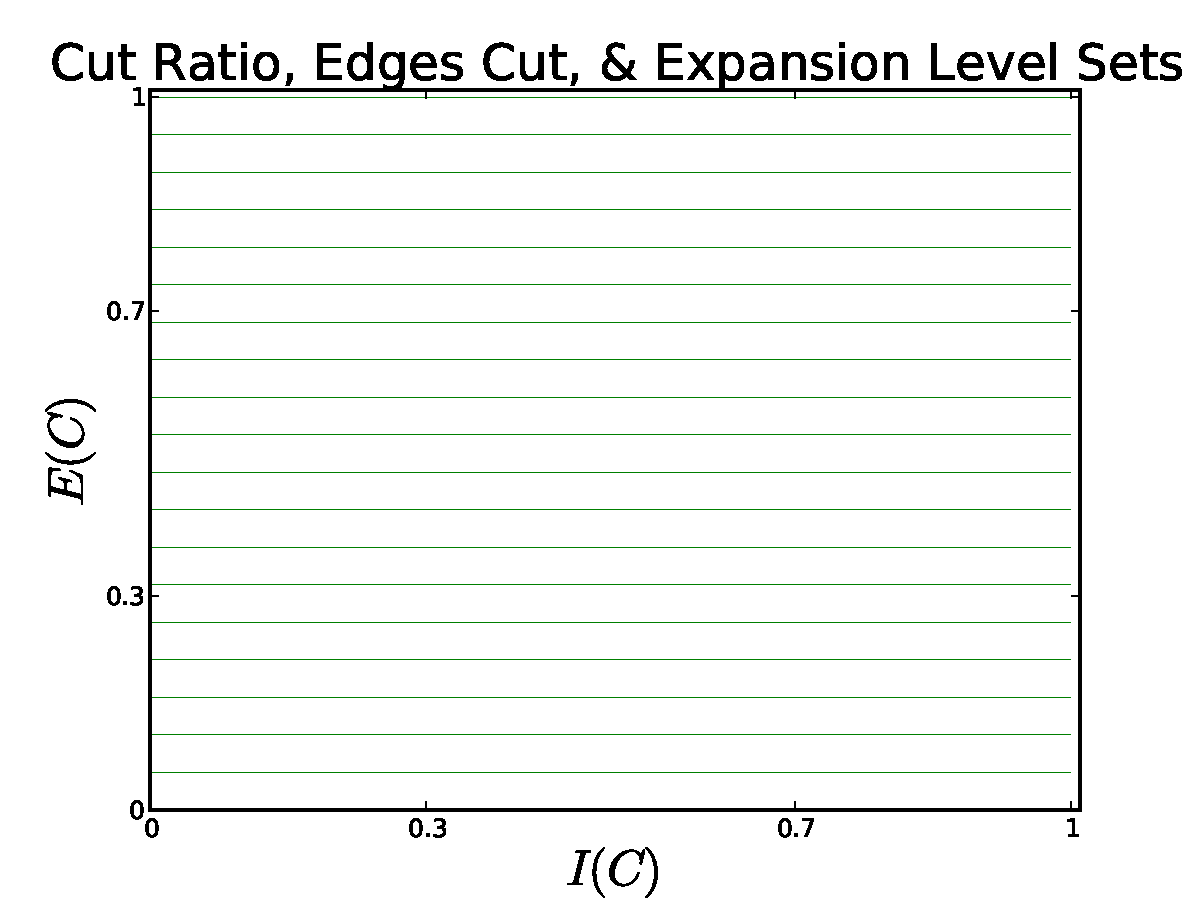
\includegraphics[width=3in]{Figures/e_based_ls}
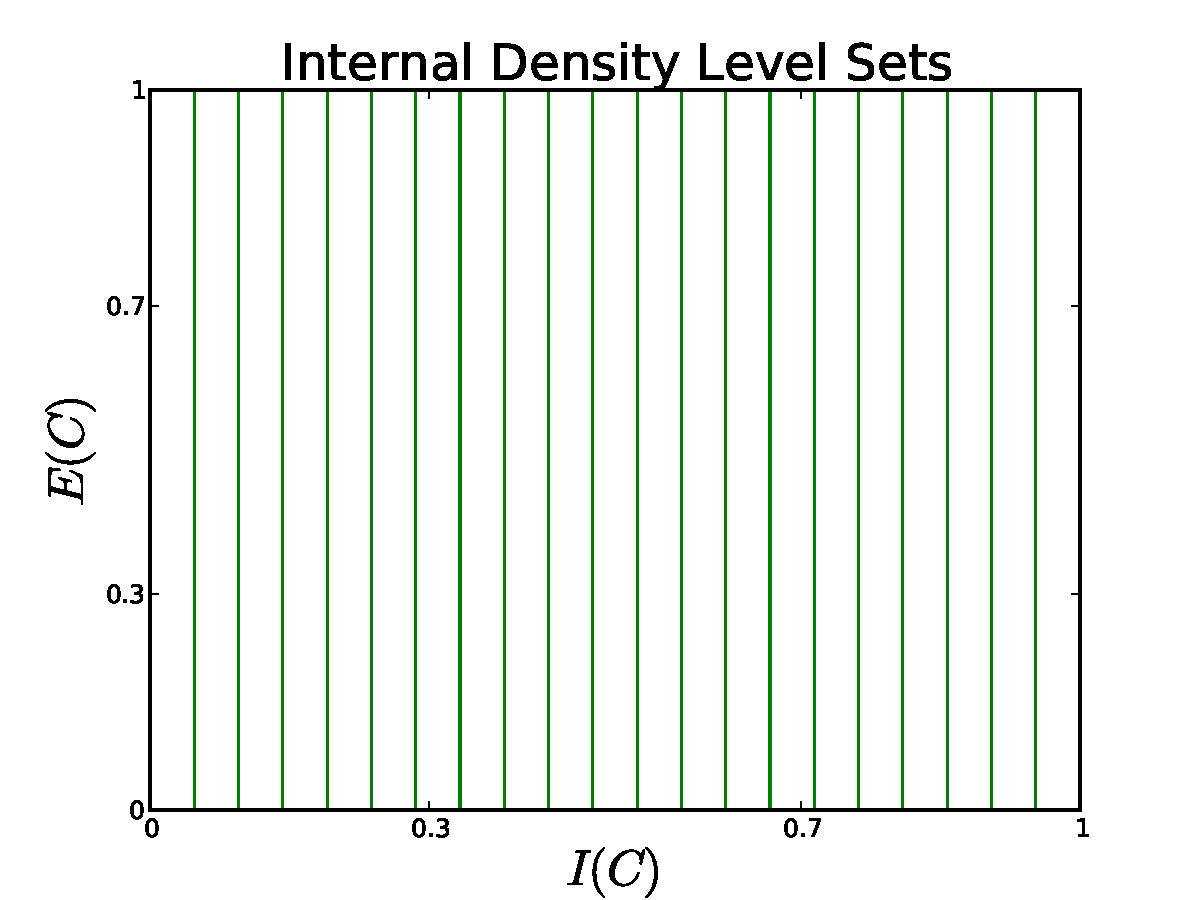
\includegraphics[width=3in]{Figures/prev_int_ls}
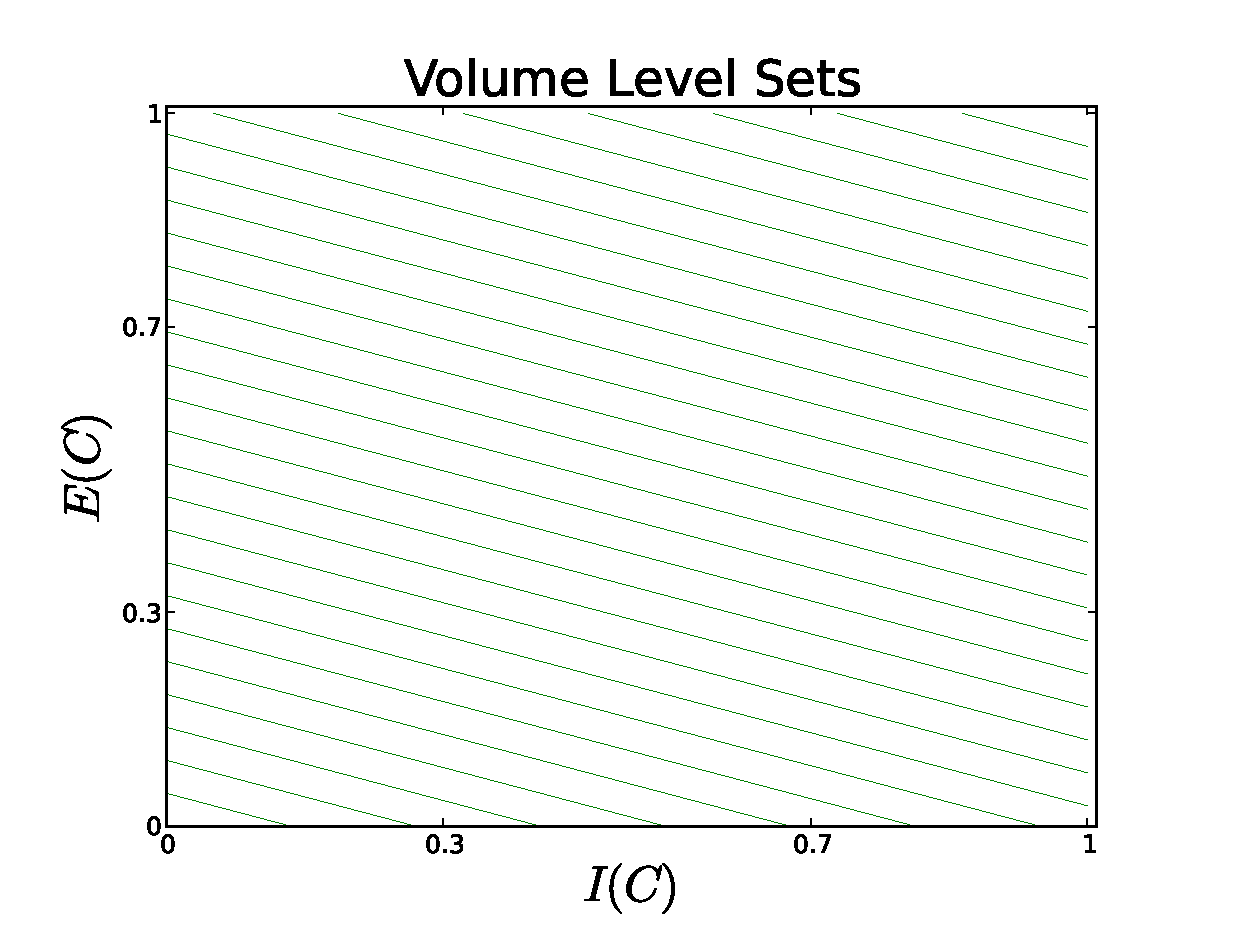
\includegraphics[width=3in]{Figures/volume_ls}
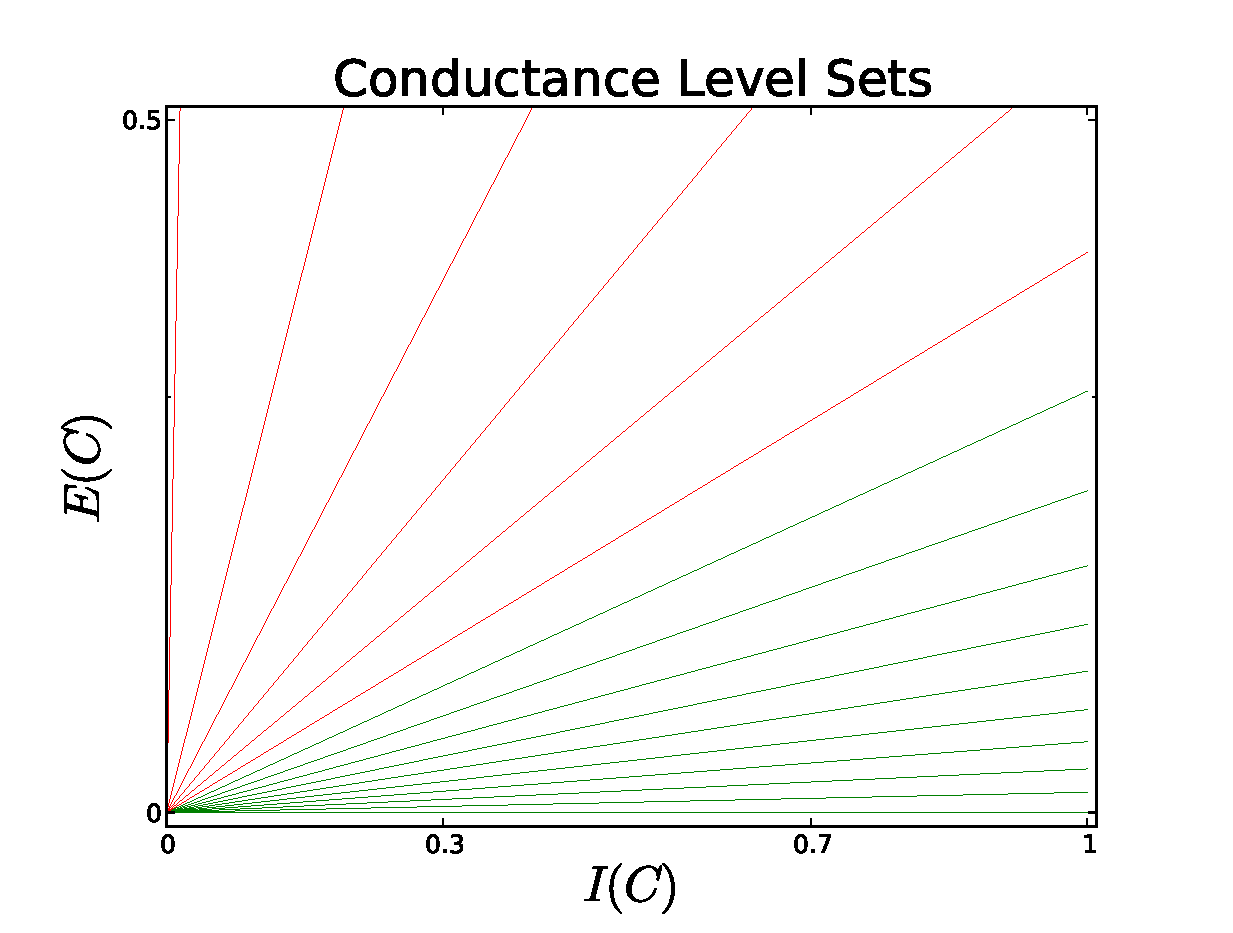
\includegraphics[width=3in]{Figures/cond_ls}
\caption{Level Sets in the $(I, E)$ plane for different metrics of a single community.}
\label{fig_single_ls}
\end{figure}

\begin{table}[!h]
\centering
\begin{tabular}{|c | c  c  |}
 \hline Metric & Optimal $C$ & $(I(C), E(C))$ \\ \hline
{\sc Conductance} & $G$& $(x, 0)$\\ \hline
{\sc Cut Ratio}  & $G$ & $(x, 0)$\\ \hline
{\sc Edges Cut}  & $G$& $(x, 0)$ \\ \hline
{\sc Expansion}  & $G$&$(x, 0)$ \\ \hline
{\sc Internal Density}  & any clique & $(1, x)$ \\ \hline
{\sc Volume}  & $G$& $(x, 0)$ \\ \hline
\end{tabular}
\caption{Communities that optimize each metric.  A value of $x$, indicates that the optimization is independent of that value.}
\label{tbl_single_optimal_communities}
\end{table}

% subsubsection*************************************
\subsubsection{Greedy Algorithm}

The simple greedy algorithm is an expansion of the community, greedily engulfing the node that improves a given {\sc Metric} the most. The algorithm is the {\it Greedy Single Community Metric Optimization} Algorithm: \ref{alg_greedy_single}.
\begin{algorithm}                              % enter the algorithm environment
\caption{{\sc Greedy Single Community Metric Optimization}}         % give the algorithm a caption
\label{alg_greedy_single}                                   % and a label for \ref{} commands later in the document
\begin{algorithmic}                        % enter the algorithmic environment
\REQUIRE $C$, $G=(V, E)$, and {\sc Metric}
\STATE $inc = 1$
\WHILE{$inc \geq 0$ and $C \neq V$}
\STATE Let $u \in V$ maximize {\sc Metric}$(C \cup u)$.
\STATE $inc \leftarrow$ {\sc Metric}$(C \cup u) - $ {\sc Metric}$(C)$
\STATE $C \leftarrow C \cup u$
\ENDWHILE
\RETURN $S$
\end{algorithmic}
\end{algorithm}

Some metrics require minimization rather than maximization, this algorithm is easily adapted accordingly.
For each metric we start the algorithm with a simple subset of two connected nodes and track the communities that result in improvements, according to a given metric. As the algorithm expands the community, the metric determines which node is optimal at each step. We record this better community and for each metric, $M$, get a set of $C_1 \subset C_2 \subset \dots \subset C_n$, such that the metric is increasing $M(C_i) < M(C_{i+1})$. While this is not an encompassing algorithm as it can only find local maximums, it will reveal a metric’s biasenesses toward communities of certain $I(C)$, $E(C)$, values.

% subsubsection*************************************
\subsubsection{Expansion, Edges Cut, and Cut Ratio}

Let us look at how $E(C)$ based metrics categorize the $(I, E)$ plane.  The metrics in this category are {\sc Expansion}, {\sc Edges Cut}, and {\sc Cut Ratio}.  We can visualize how the plane is viewed by these metrics with level sets.  For all points of the $I,E$ plane, we evaluate the metric and graph the contour curves, or level sets\cite{}.  In level set figures, any two points in the $I,E$ plane connected by a curve have the same metric value. In our Greedy Algorithm \ref{alg_greedy_single}, if the algorithm can add a node to the community that crosses a level set to a higher metric valuation the algorithm will add that node.  Visually, the more level sets crossed by a change to the community, corresponds to a higher change in the metric.  Traditionally, level sets are used in this manner to show gradient descent to find a local minimum.  The optimum that a gradient descent will find, can be found by traveling perpendicular to the level sets.  While we find in practice this is a good analogy to understand the behavior of optimizing these metrics,  we can not quite finish the analogy as the metrics are discrete.  Hence, we can not quite use level sets to compute communities.  But, we can use level sets as a visual categorization of the $(I, E)$ plane according to a metric.


The level sets of cut ratio, edge cuts, and expansion, fFgure \ref{fig_corner_sets}, across the $I,E$ plane reveal the $I,E$ values of the communities that optimize these metrics.  While, the three metrics have different definitions, their level sets are identical only with different values.  The level sets are horizontal lines, whose metric's are optimized by improvements in $E(C)$, irregardless of changes to $I(C)$.  Accordingly, the node that has the greatest improvement in $E(C)$ is the same for all three metrics, and each metric results in the same path through the $I,E$ plane.


Though it does not make a difference in our examples, the difference between these metrics is their treatment of $k = \frac{|C|}{|V|}$.  Cut ratio is unresponsive to changes in the size of the community, while expansion linearly discounts against larger communities.  Edges cut heavily favors very large or very small communities.  See {\it Fig. \ref{fig_k_e_based}}

\begin{figure}[!h]
\centering
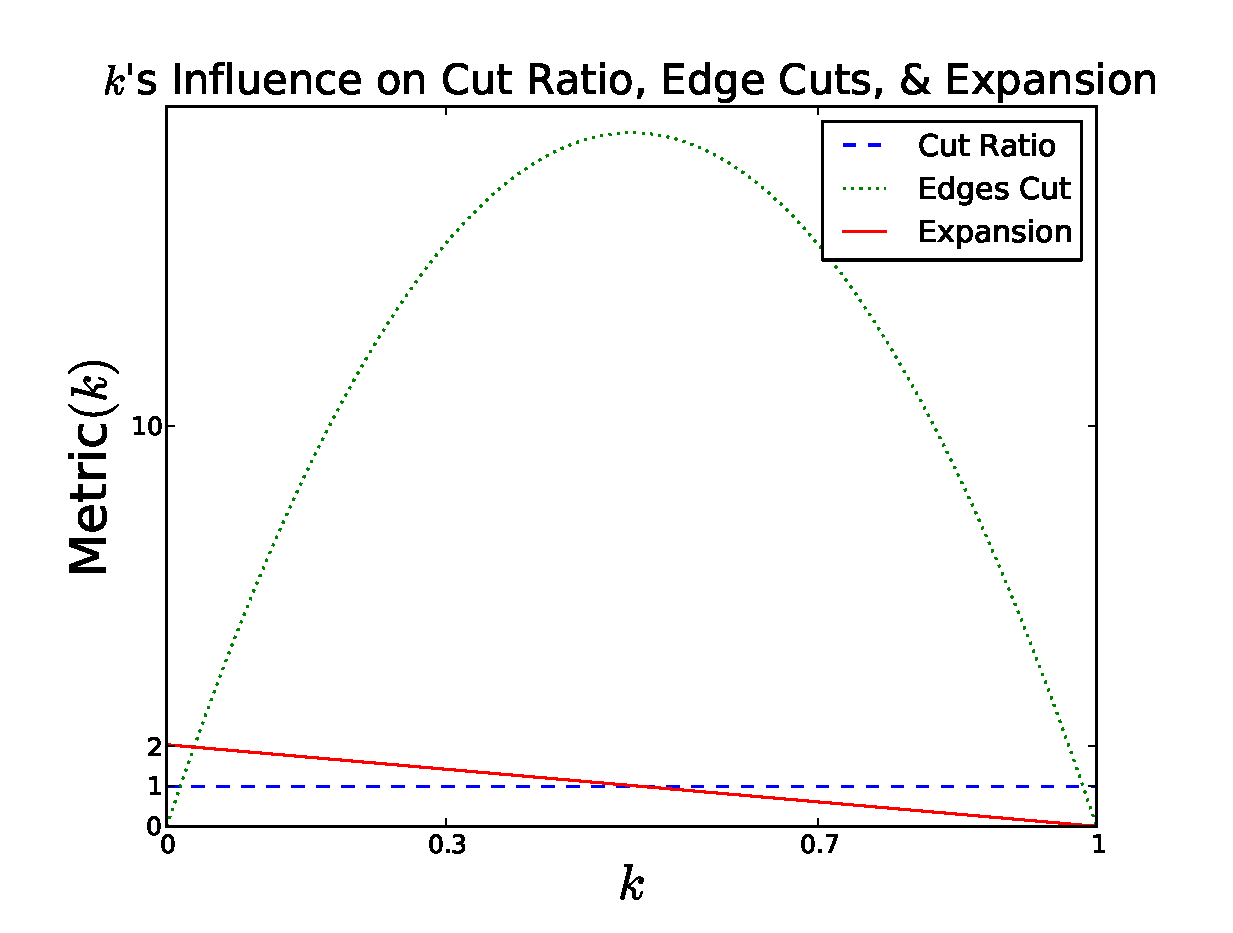
\includegraphics[width=4in]{Figures/k_influence_e_based}
\caption{Influence of size of community on the values of external density based metrics.}
\label{fig_k_e_based}
\end{figure}


\begin{figure}[!h]
\centering
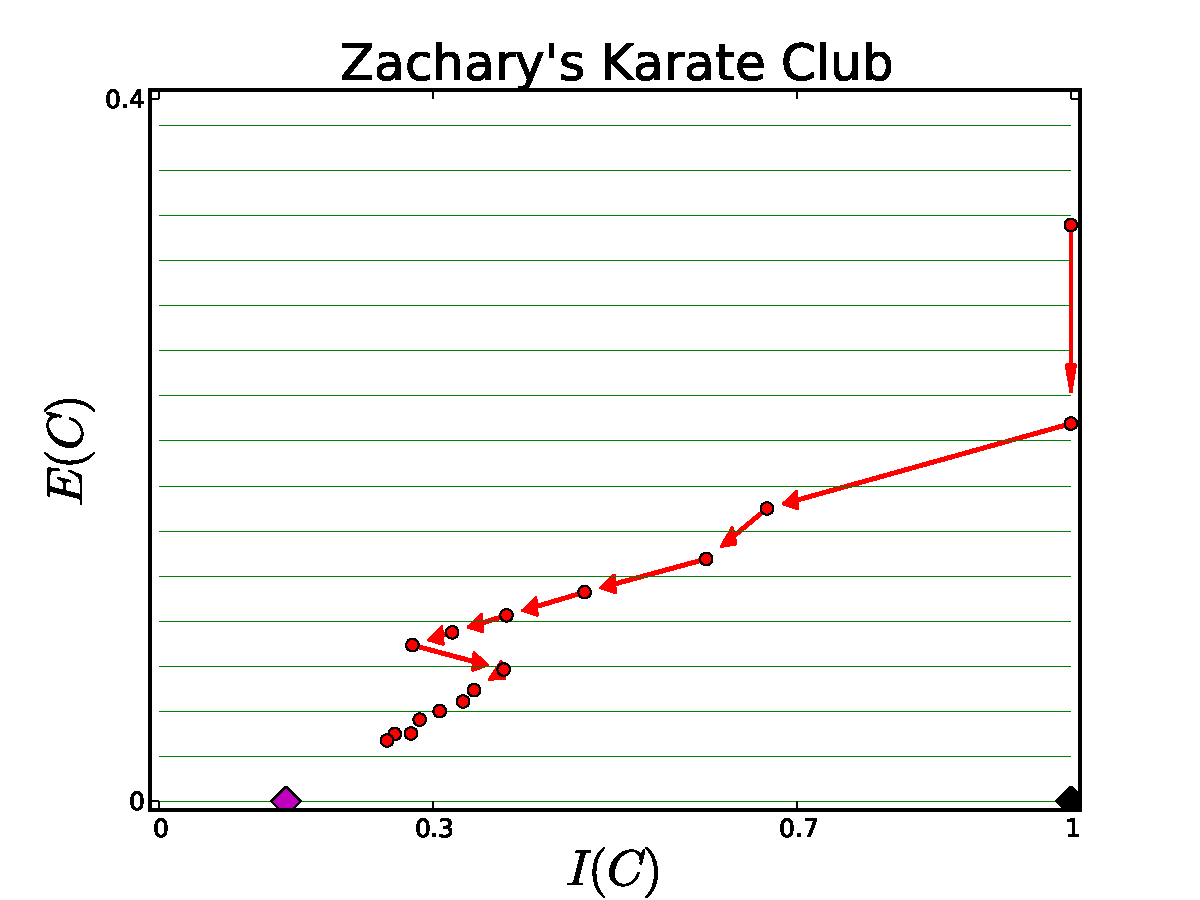
\includegraphics[width=2.8in]{Figures/cee_karate}
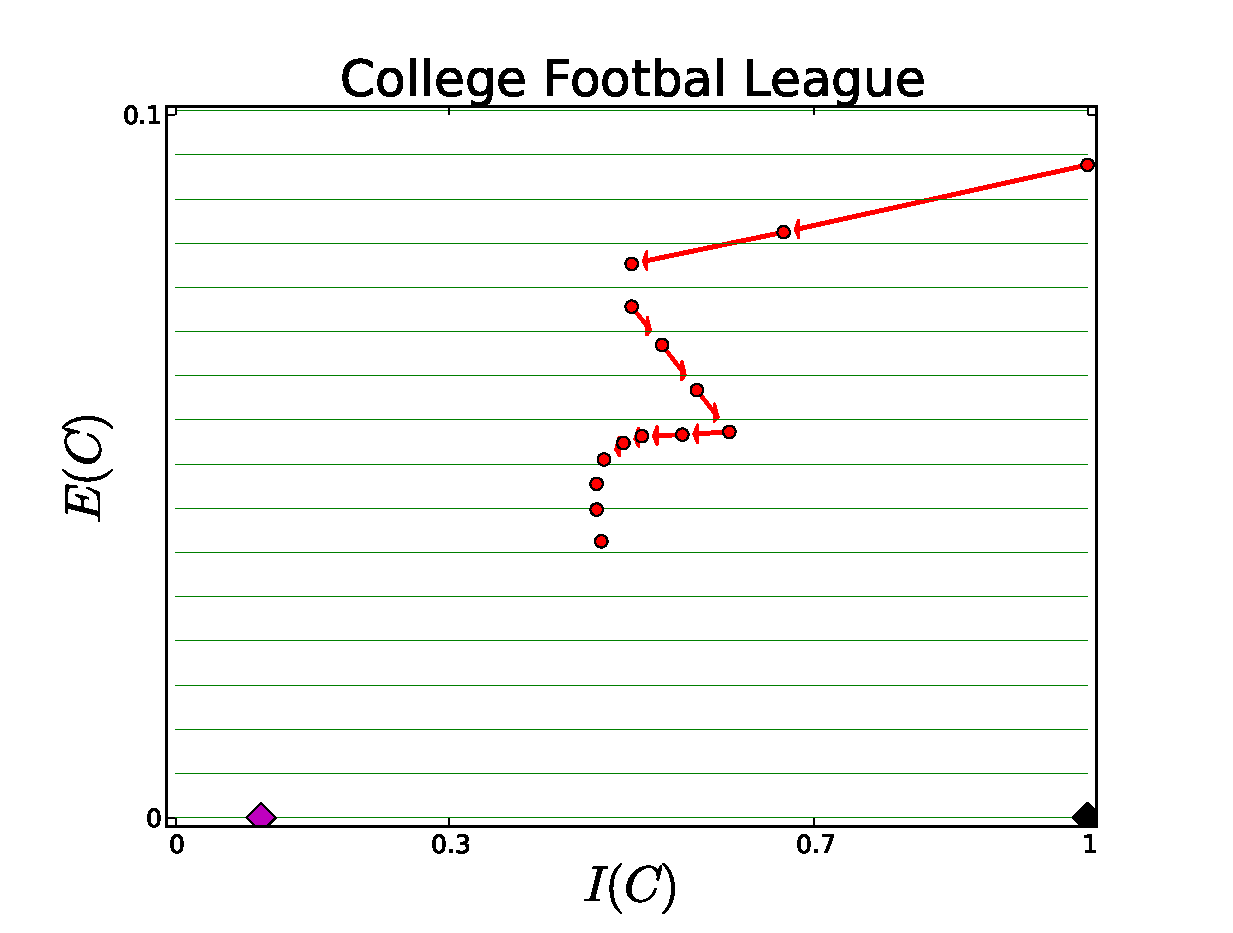
\includegraphics[width=2.8in]{Figures/cee_cfl}
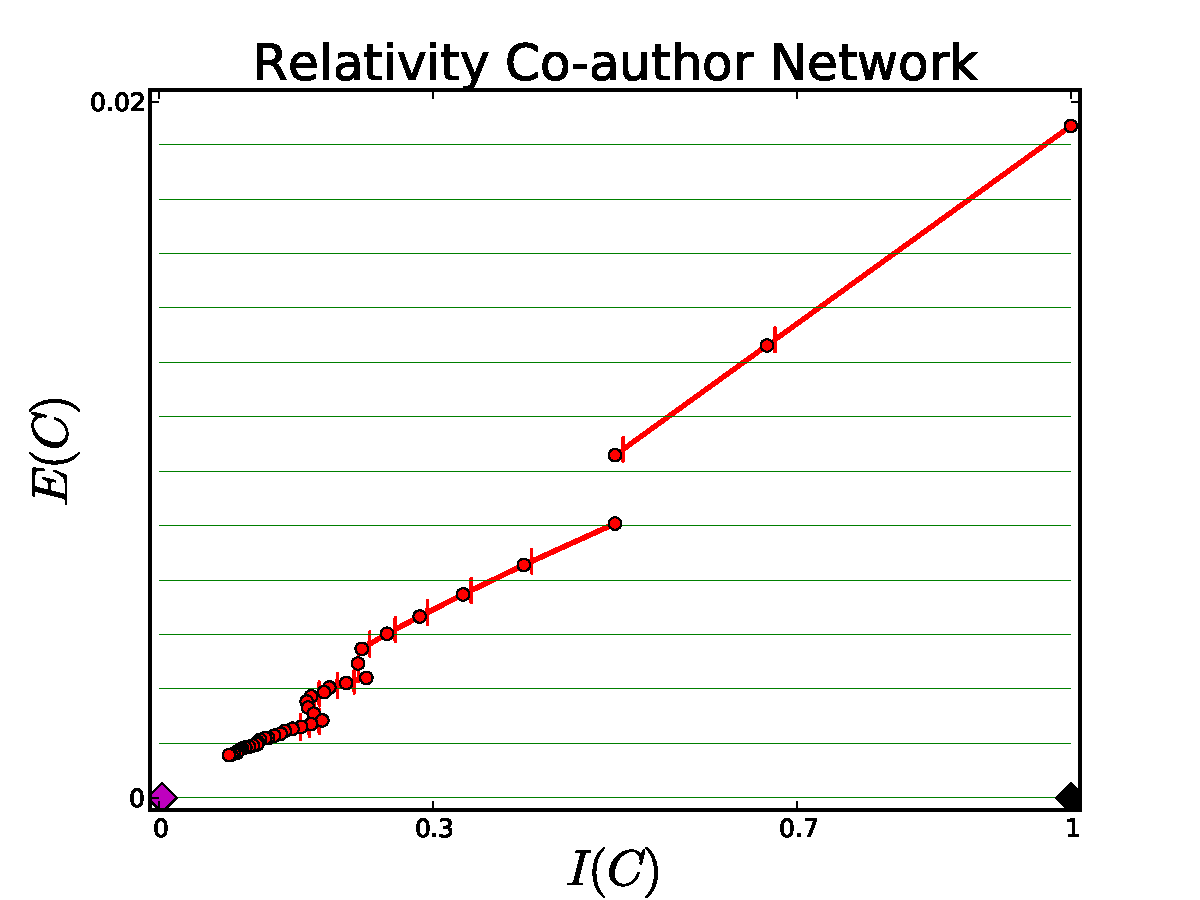
\includegraphics[width=2.8in]{Figures/cee_relativity}
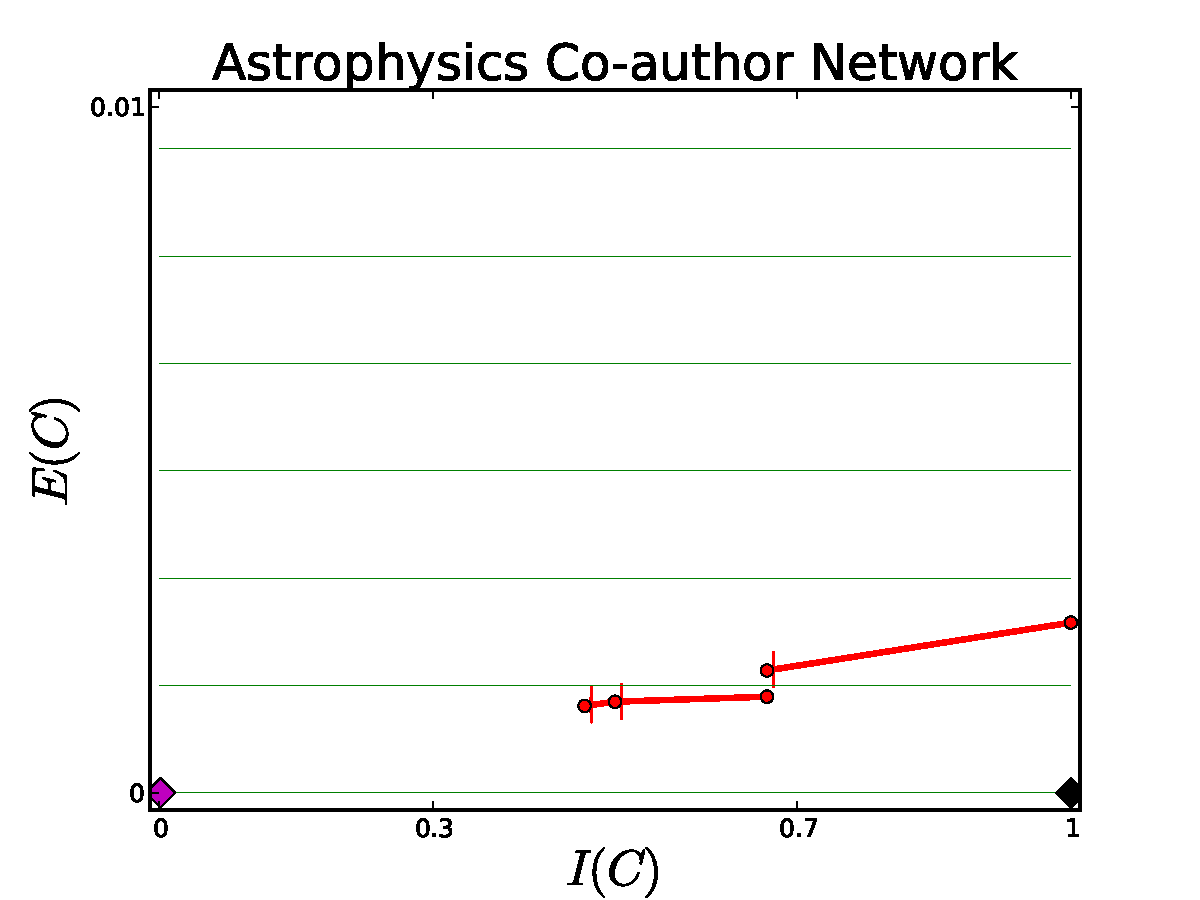
\includegraphics[width=2.8in]{Figures/cee_astro}
\caption{External Density based metrics({\sc Cut Ratio}, {\sc Edges Cut}, and {\sc Expansion}) optimized in different networks.  The lower left diamond is the $(I(C), E(C))$ point corresponding to a community of the entire graph.  The lower right diamond is the $(I(C), E(C))$ point corresponding to an ideal community.  The path corresponds to the intermediatory $(I, E)$ values of adding nodes that optimize the metrics using Greedy Algorithm \ref{alg_greedy_single}}
\label{fig_real_e_based}
\end{figure}




% subsubsection*************************************
\subsubsection{Internal Density as previously defined}

On the polar extreme of cut ratio, edge cuts, and expansion, is internal density.  Internal density is a function of internal density and is unresponsive to changes in the the external density.  We do not include indepth analysis, but rather a summary.  The level sets of internal density are vertical lines in the $I,E$ plane.  The paths produced by the greedy algorithm grow out the original community to the largest clique it can find(if forced to), as the internal density of two connected notes is already maximal.  Any clique is an optimization of internal density, irregardless of external connectivity.


% subsubsection*************************************
\subsubsection{Volume}

\begin{figure}[!h]
\centering
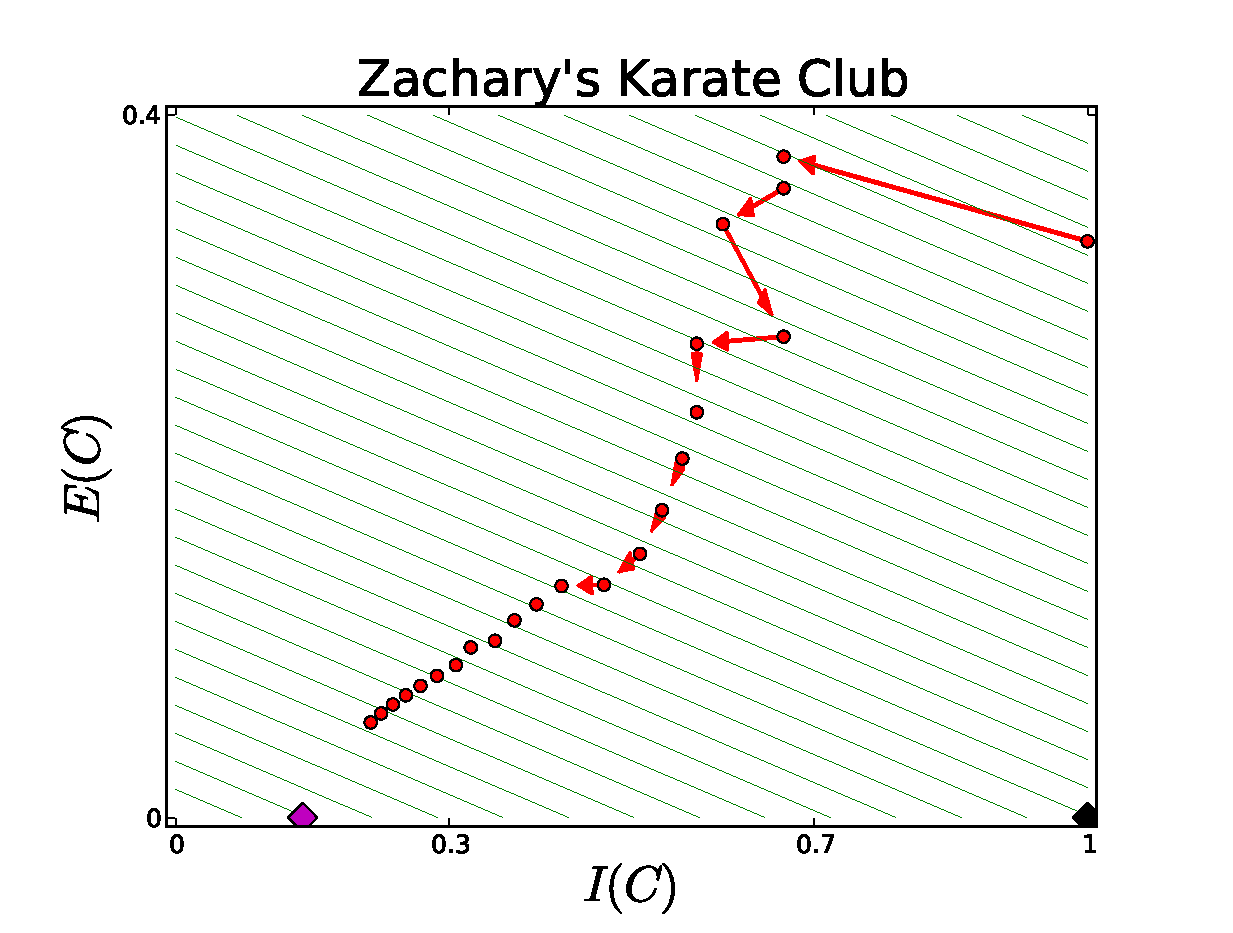
\includegraphics[width=2.8in]{Figures/volume_karate}
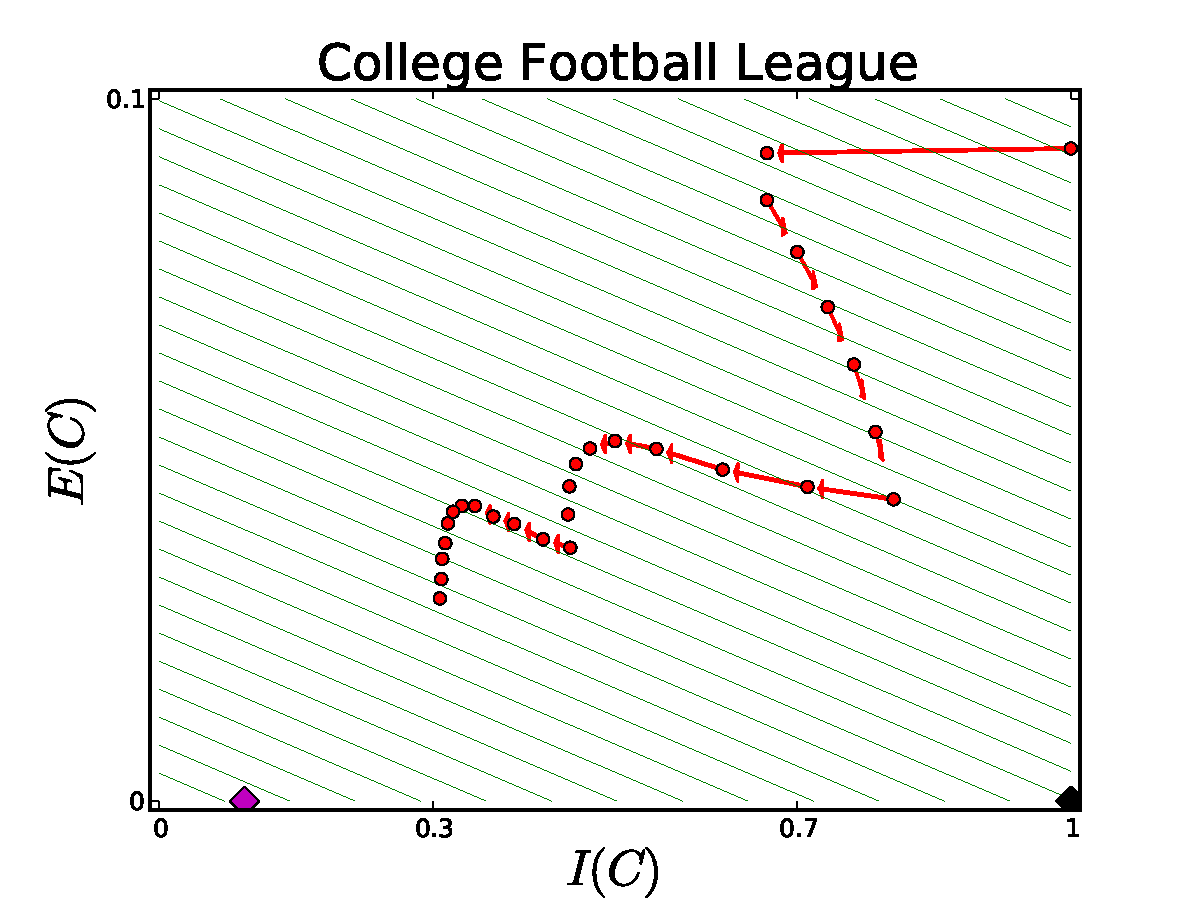
\includegraphics[width=2.8in]{Figures/volume_cfl}
\caption{Tracing of communities found by volume through the IE plane.  The paths are much longer, extending until the community includes the entire graph.  We cut the paths short once they progress towards including the entire community.  The lower left diamond is the $(I(C), E(C))$ point corresponding to a community of the entire graph.  The lower right diamond is the $(I(C), E(C))$ point corresponding to an ideal community.  The path corresponds to the intermediatory $(I, E)$ values of adding nodes that optimize the metrics using Greedy Algorithm \ref{alg_greedy_single}.}
\label{fig_real_volume}
\end{figure}

A metric that takes both internal and external density into account is volume.  The next conclusion is not apparent just from the equation parameterized in terms of internal and external density.  However, observing the level sets of volume reveal that the optimal community is at $(I, E) = (0, 0)$ and volume as a metric is optimal for communities with low external density and low internal density.  Apart from communities of disconnected nodes, volume can best be optimized by a community encompassing the entire graph.  Volume directly contradicts our intuition that communities should have good internal connectivity.

\begin{figure}[!h]
\centering
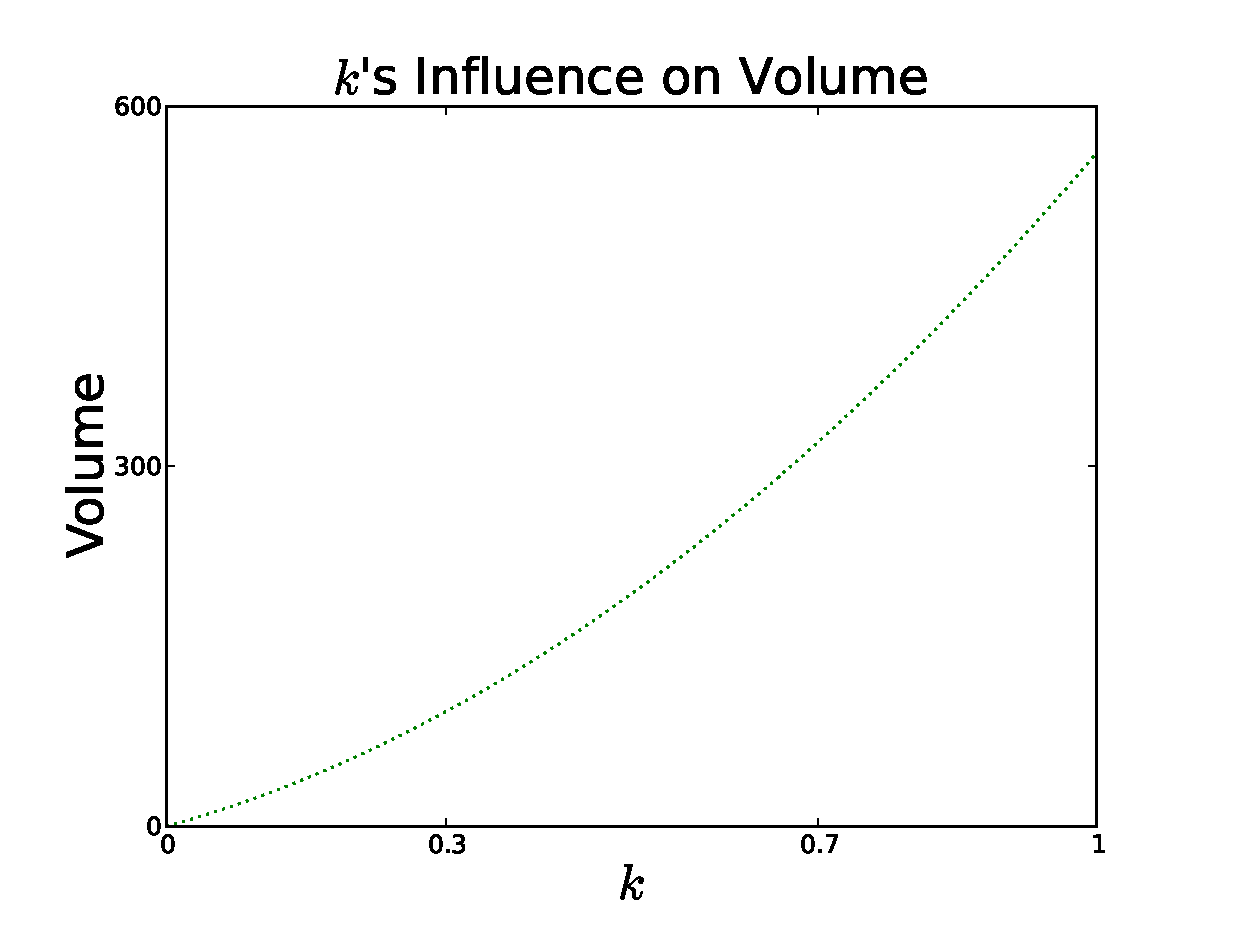
\includegraphics[width=2.8in]{Figures/volume_k}
\caption{The affect, increasing the size of the community has on volume, even for a constant $I(C)$ and $E(C)$.}
\label{fig_volume_k}
\end{figure}


% subsubsection*************************************
\subsubsection{Conductance}
For conductance the level sets are rays radiating from $(I, E) = (0, 0)$, see {\it Fig. \ref{fig_single_ls}}.  As the rays become closer to horizontal, $E = 0$, conductance becomes optimal.  Hence, no matter the data set, conductance desires communities with $I,E$ values closer to $(I,E) = (x, 0)$, for any arbitrary $I(C) = x$.  Including more nodes that continually increase $I(C)$ is rare in networks and much more common is decreasing $E(C)$ by encompassing more of the graph.  Since, conductance is fairly, unresponsive to changes in $I(C)$, optimizing conductance results decreasing $E(C)$ as much as possible.  How much conductance is biased towards small improvements in $E(C)$ verse large improvements in $I(C)$ depends on where in the $I,E$ domain the seed communities originate.   In the College Football League, the seed community begins a portion of the domain where improvements in $I$ and $E$ are balanced.  For Zarchary's Karate Club, the seed community quickly falls into a portion of the $I,E$ domain where small and easy improvements in $E$ benefit conductance more than large and hard changes in $I$.

\begin{figure}[!h]
\centering
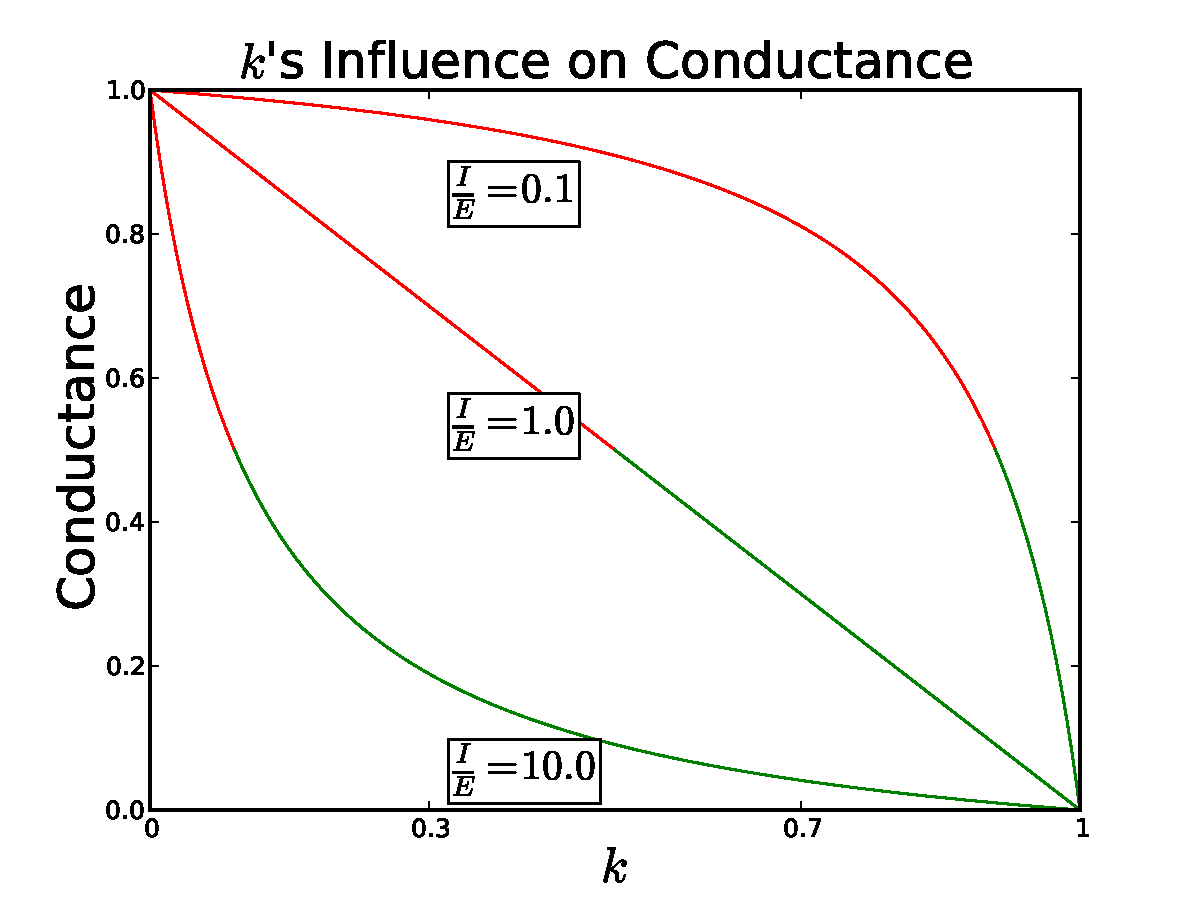
\includegraphics[width=4in]{Figures/k_influence_conductance}
\caption{Influence of size of community on the value of conductance.}
\label{fig_k_conductance}
\end{figure}

The last parameter that must be taken into account is $k$, the proportion of the graph covered by the community.  Now we fix the $I, E$ ratio and observe how changes in $|C| = k |V|$ affect conductance.  The conclusion,   If the expansion of the community is greatly affected by $k$, then our previous analysis will yield to conductance favoring the largest possible community as demonstrated in {\it Fig. \ref{fig_k_conductance}}.  This affect can be seen in the change of $C_1$ to $C_2$ in the plotted paths in {\it Fig. \ref{fig_conductance_karate}}, as the relative size change of adding just one node is large.

That conductance favors large disconnected communities, even with low internal density, is experimentally confirmed by \cite{}.  However, as long as the community is of medium size and has a much larger $I(C)$ value than $E(C)$ conductance will make improvements that correspond to our intuition that an ideal community is internal dense and externally sparse.

\begin{figure}[!h]
\centering
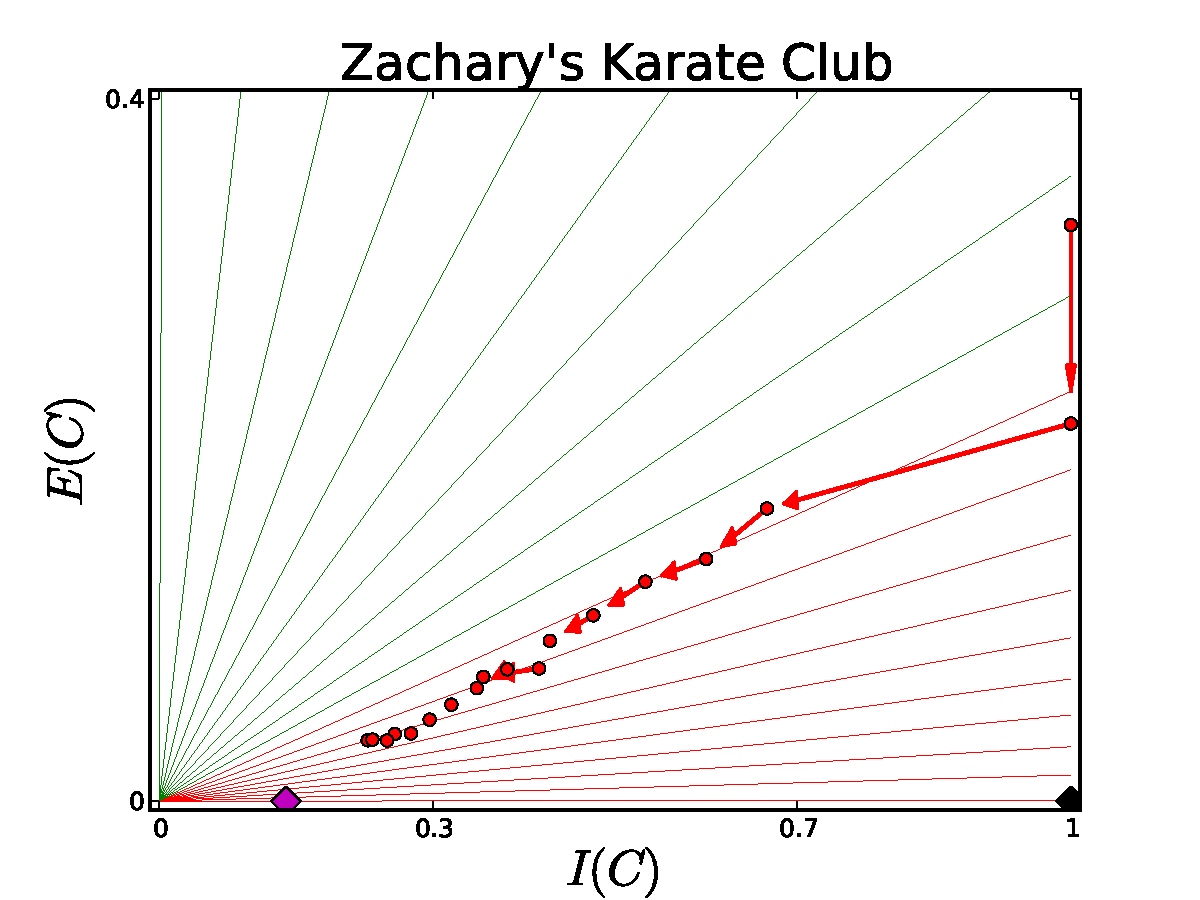
\includegraphics[width=2.8in]{Figures/conductance_karate}
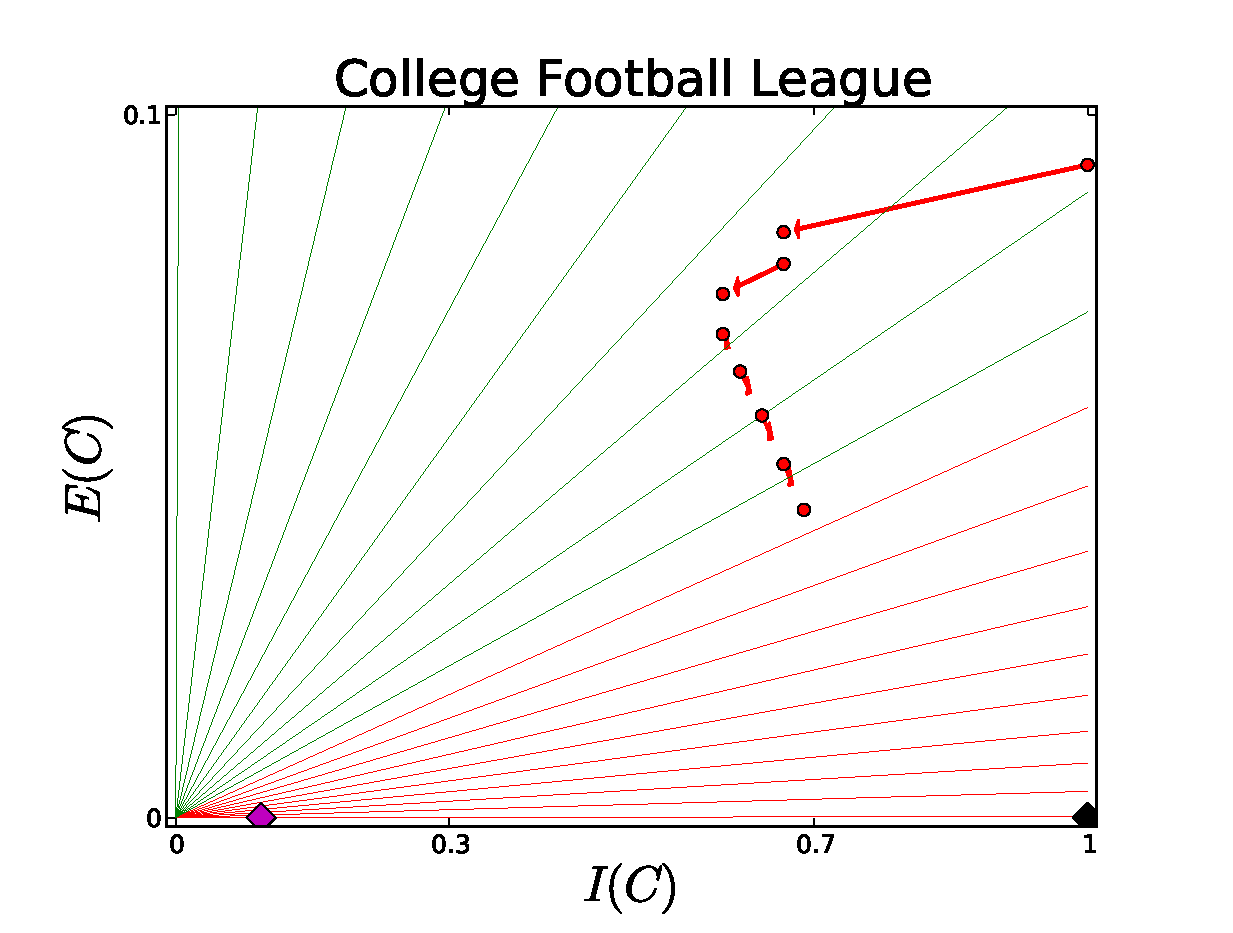
\includegraphics[width=2.8in]{Figures/conductance_cfl}
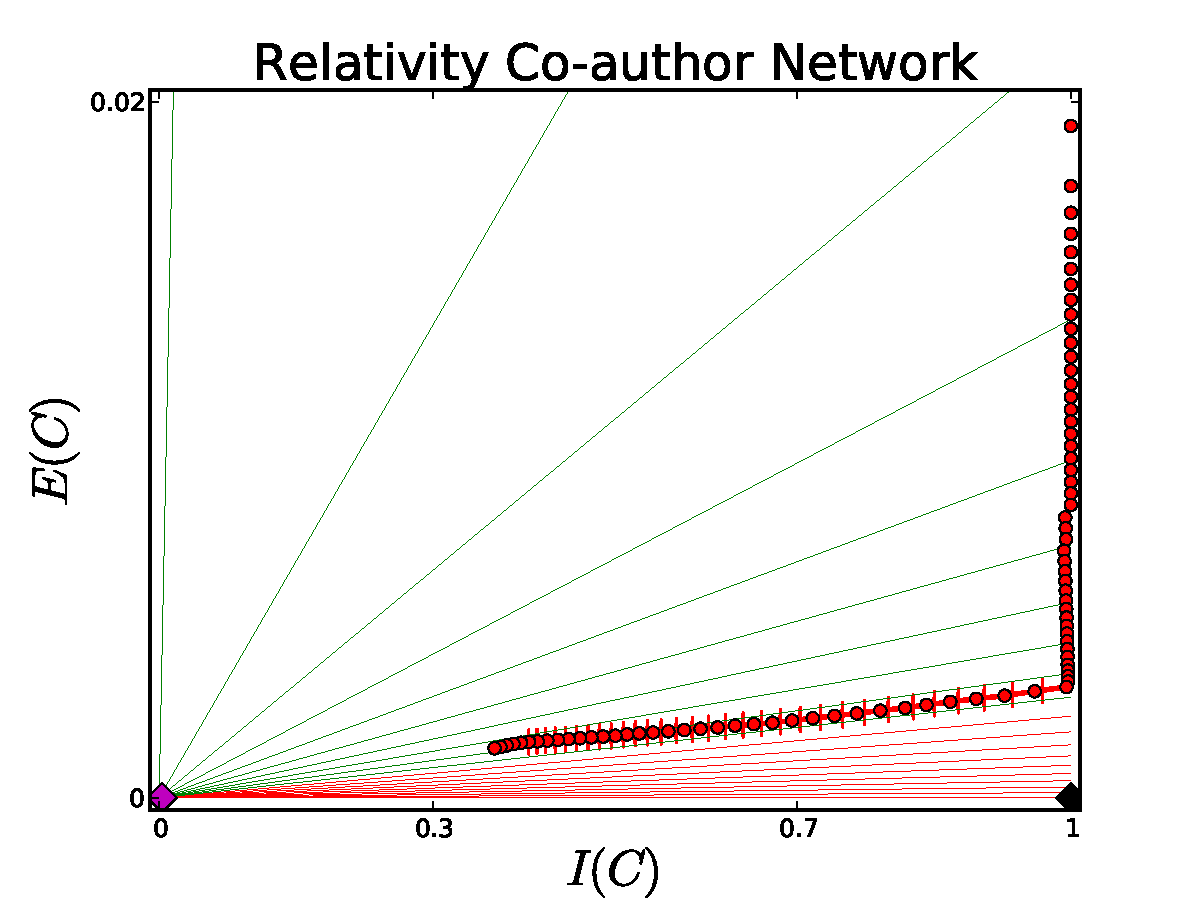
\includegraphics[width=2.8in]{Figures/conductance_relativity}
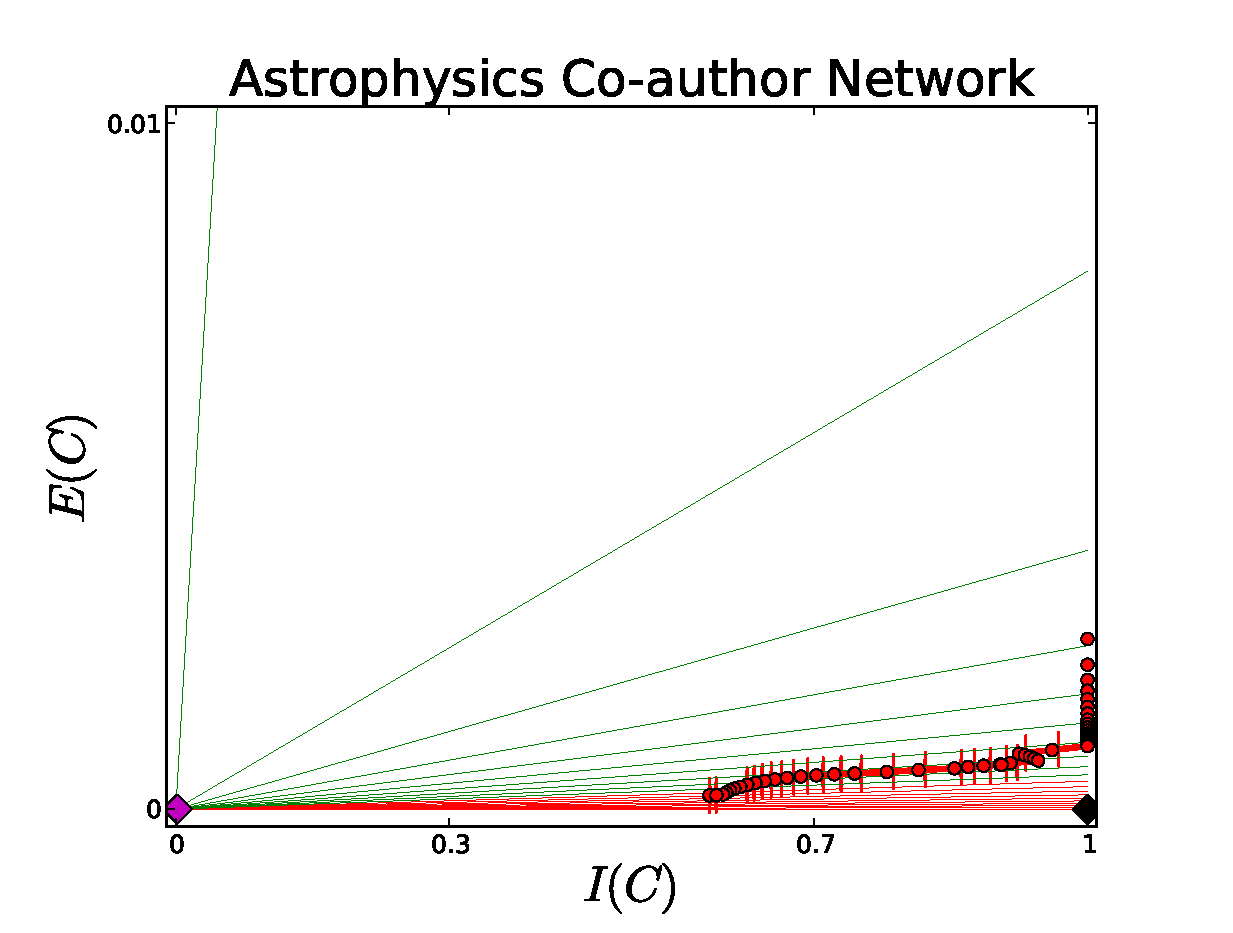
\includegraphics[width=2.8in]{Figures/conductance_astro}
\caption{The progression of communities that optimize conductance.  Note, the entire graph optimizes conductance, we stop following the progression of conductance once it becomes obvious the entire graph will be engulfed. (In the case of the college football league, a local optimum was reached.)}
\label{fig_real_e_based}
\end{figure}


% New Section******************************
\section{Set of Communities Based Metrics}

We now explore metrics that evaluate the strength of a set of communities.  A majority of these community detection methods are based on finding a partitioning of the network into communities.  For a given network, community detection produces a set of communities, $S$, where each node $u$ belongs to exactly one community, $C_i \in S$.  The most popular of these detection methods is, maximizing modularity \cite{}.  Modularity returns a single valued evaluation of a set of communities.

As with individual community based metrics, we will develop an understanding of the pertinent parameters of a set of communities.  Through these parameters, there exist some closed form parameterizations for metrics on sets of communities.  Primarily, though, we will build the space of these parameters that a set of communities may evaluate to and analyze how these metrics valuate communities of different parameters.  Again, our conclusions are independent of a specific network.


% New Subsection **********************************************
\subsection{Internal Density, External Density, and Conciseness}

Our parameterization of internal and external density for single community metrics can not be directly applied to a set of communities, $S = \{C_1,C_2,...C_n\}$. Though if we follow the same logic we will arrive at a similar parameterization. An ideal set of communities are cliques such that every edge is within some community. In addition, the community description of the network should not have an exponential number of communities, but rather some concise set of communities. Hence an ideal set of communities has three parameters. Internal density is a representation of how close the set of communities is to being a set of cliques. External density is a representation of how close the set of communities are to covering all edges in the graph. Size of the set of communities is a representation of how concise the set of communities are. With the same methodology for parameterizing and understanding metrics of individual communities we proceed to parameterize metrics for sets of communities with {\it internal density}, {\it external density}, and {\it conciseness}.  Formal definitions follow.

\begin{definition}[Internal Density of a Set of Communities] For a set of communities, $S = \{C_1, C_2, \dots, C_n\}$, the internal density of the set is ratio between the sum of the number of edges that do exist within each community to the maximal value of that sum.  The maximal value is achieved by all communities being cliques.
\begin{equation}
I(S) = \sum_{C \in S} \frac{\sum_{u \in C} \sum_{v \in C} w(u,v)}{\sum_{C \in S}|C|(|C| - 1)}
\end{equation}
\label{def_int_set}
\end{definition}

\begin{definition}[External Density of a Set of Communities] In a set of communities $S$, the {\sc Ext\_Edges} are the edges, not covered by any community.  Hence, external density is the fraction of edges not covered by any community.
\begin{equation}
E(S) = \frac{\sum_{(u, v) \in \mbox{\sc Ext\_Edges}} w(u,v)} {\sum_{u,v \in V}w(u,v)}
\end{equation}
\label{def_ext_set}
\end{definition}

\begin{definition}[Conciseness of a Set of Communities]  Conciseness is the size of the description necessary to describe all of the communities.
\begin{equation}
\mbox{\sc Conciseness}(S) = |S|
\end{equation}
\label{def_conciseness}
\end{definition}

An useful byproduct of our choice of defining the parameters, is the ability to analyze, any set of communities, including overlapping communities.  Our definition of internal density for a set of communities, allows nodes to be placed in multiple communities, but insists that a high internal density corresponds to a node being well connected to all communities it belongs to.  External density is independent of overlapping communities, as well as conciseness.

To date we do not know of any previous metrics that have a closed form parameterization in terms of $I(S)$, $E(S)$, and $|S|$. We release a linear metric pertaining to these parameters in a later section.
\begin{definition}[Ideal Set of Communities]
A set of communities, $S$, is ideal if it is a set of cliques that cover the graph in the fewest necessary communities:
\begin{eqnarray*}
I(S) &=& 1\\
 E(S) &=& 0 \\
|S| &=& 1.
\end{eqnarray*}
\end{definition}


All three parameters are necessary to ensure a complete description of a set of communities.  For any two parameters, there exists a set of communities that can maximize those two parameters, but not the third parameter, revealing an undesired property of the set of communities. Figure \ref{fig_corner_sets}, illustrates the types of communities that can optimize for any two parameters.

\begin{figure}[!h]
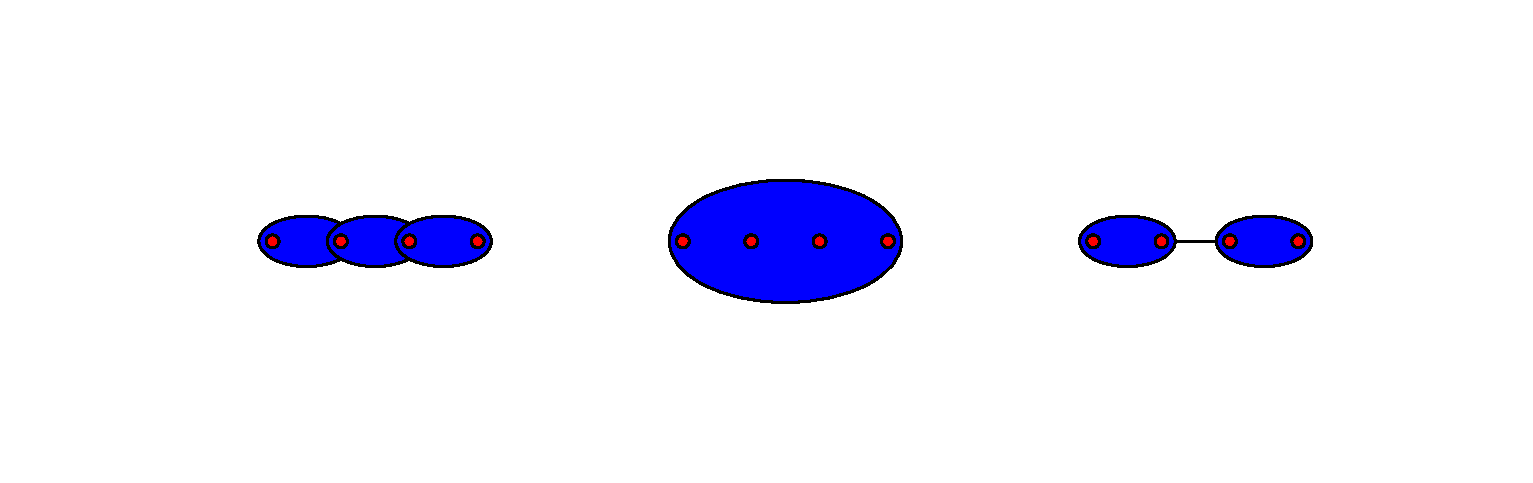
\includegraphics[width=6in]{Figures/pathological_graphs}
\caption{The communities that optimize $2$ out of $3$ parameters.  Nodes are in red, lines are edges, and communities are blue ellipses.  The left community configuration optimizes $I(S) = 1$ and $E(S) = 0$, but not conciseness at $|S| = 3$.  The middle configuration optimizes $E(S) = 0$, $|S| = 1$, but not internal density at$I(S) = \frac{1}{2}$.  The right configuration optimizes $I(S) = 1$ and nearly conciseness at $|S| = 2$, but does not optimize external density at $E(S) = \frac{1}{3}$}
\label{fig_corner_sets}
\end{figure}

% New subsection********************
\subsection{Study of Relevant Metrics}


Modularity is a partitioning of the network, and each partition is deemed a community.  For each module its modularity is the difference of the existing internal edges and expected number of internal edges, had the graph been random, with the same distribution of node degrees.  The total modularity is then the sum of the modularity of each partition.  Modularity was developed by [] and has found wide spread use due to the fast algorithms for maximizing modularity \cite{modularity}.  In particular, the use of dendograms in the Louvain Algorithm \cite{louvain} runs in minutes for large networks.

There is not a closed form parameterization of modularity in terms of our definitions of $I(S)$, $E(S)$, and $|S|$.  But we find $I(S)$ and $E(S)$ to be intuitive enough to provide the space in which to analyze metrics of sets of communities.

Still, we would like to be able to use level sets for some visual explanation of how modularity behaves with regard to some internal and external density.  The parameterization of modularity we can provide is in terms of $I(C)$ and $E(C)$ for single communities.  If we allow, $p=\frac{|C|(|C|-1)}{2L}$ and $q=\frac{|C|(|V|-|C|)}{2L}$ to be constants:
\begin{equation}
 \mbox{\sc Modularity}(S) = \sum_{C \in S} p I(C) - \left(p I(C) + q E(C)\right)^2.
\end{equation}

We can draw loose conclusions from this parameterization.  The first check is that a set of disjoint cliques are the only communities that optimize modularity.  There are no counter intuitive communities that optimize modularity.  Overall, modularity is a two part optimization.  For seed communities, in the case of modularity individual nodes, the typical initial values are high in external density.  When $E(C)$ is high it is the dominating term and the optimization is to decrease $E(C)$ as quickly as possible.  Once, external density is not the dominating term the optimization is then center around trying to improve $I(C)$.  The transition between these two phases of optimization is sudden as attested by the level sets.

We would like to recommend modularity should be designed to optimize for improvements in internal density first to find the dense cores of communities and then optimize over external density to cover more of the graph.  The reasoning is that improvements in external density can be made at any time by increasing the size of communities.  However, improvements in internal density can only be made while the communities are small and closer to cliques.

\begin{figure}[!h]
\centering
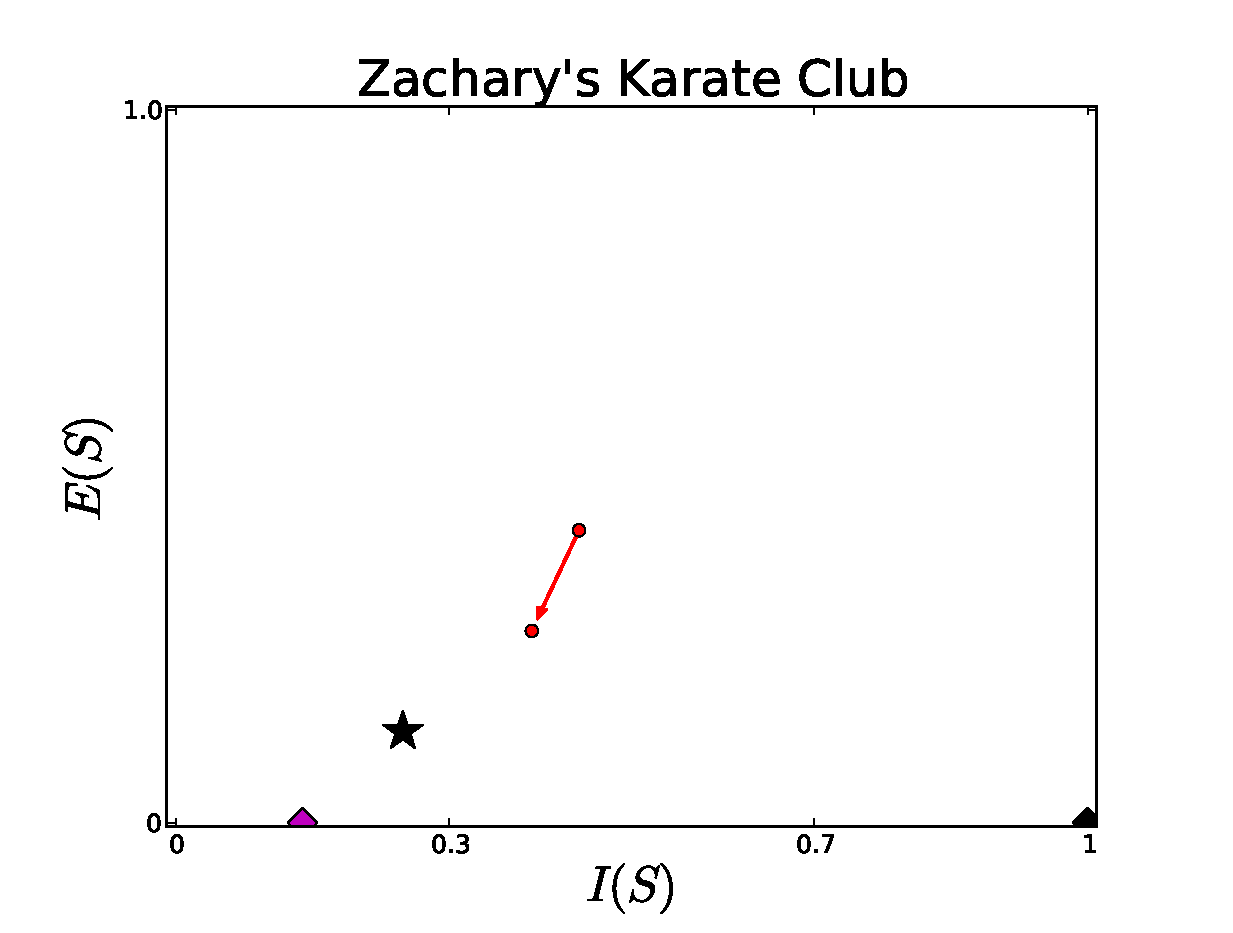
\includegraphics[width=2.8in]{Figures/modularity_karate_sets}
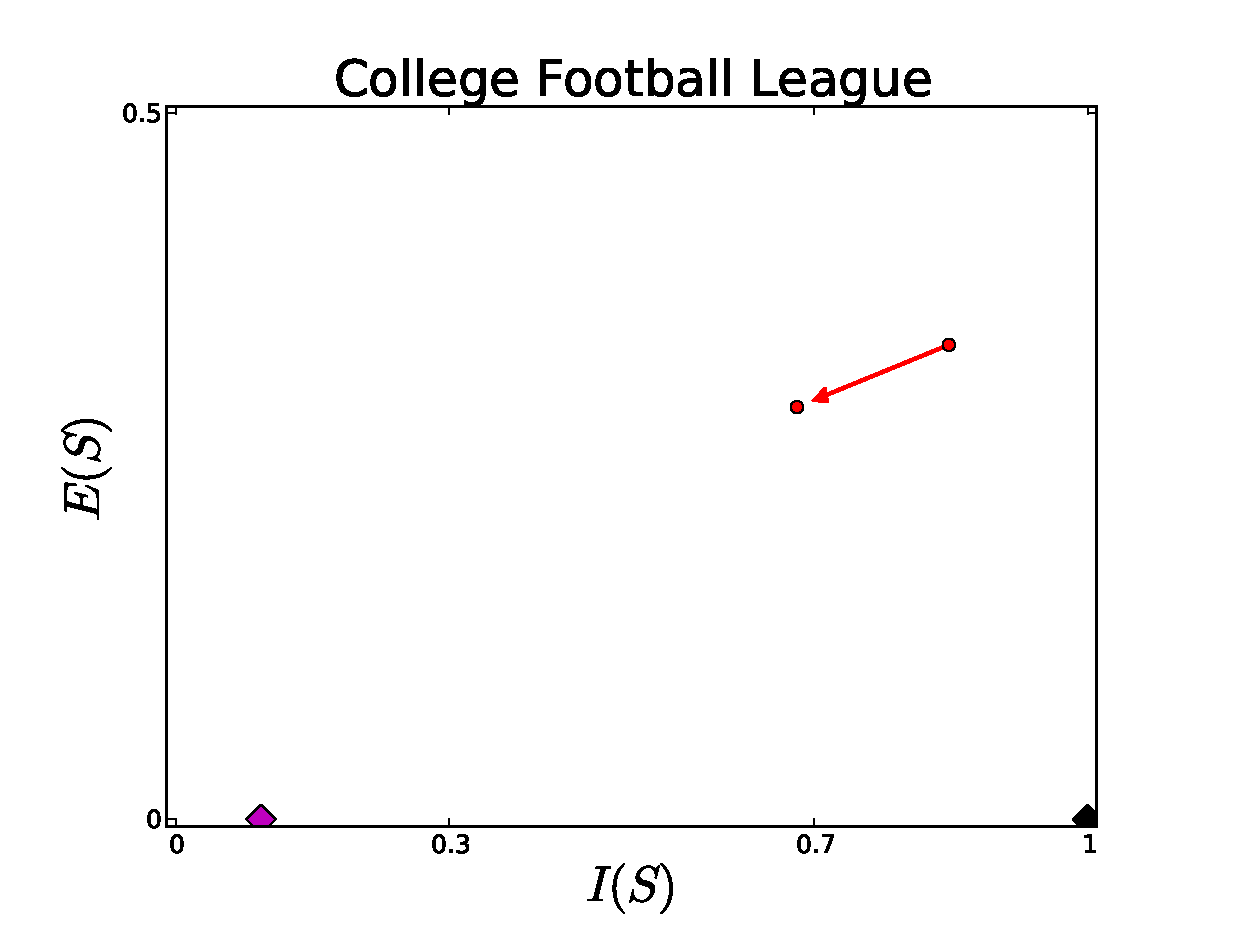
\includegraphics[width=2.8in]{Figures/modularity_cfl_sets}
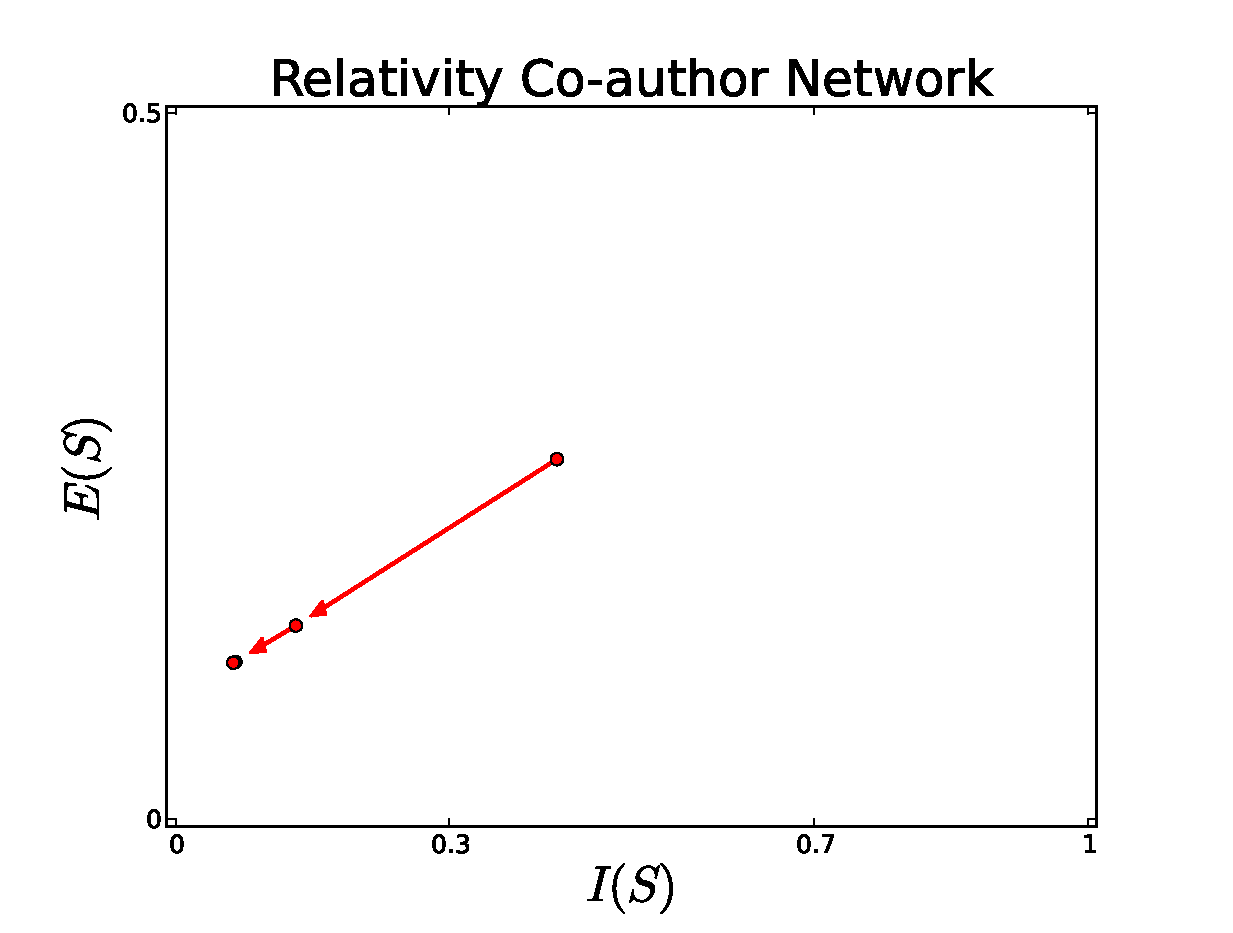
\includegraphics[width=2.8in]{Figures/modularity_relativity_sets}
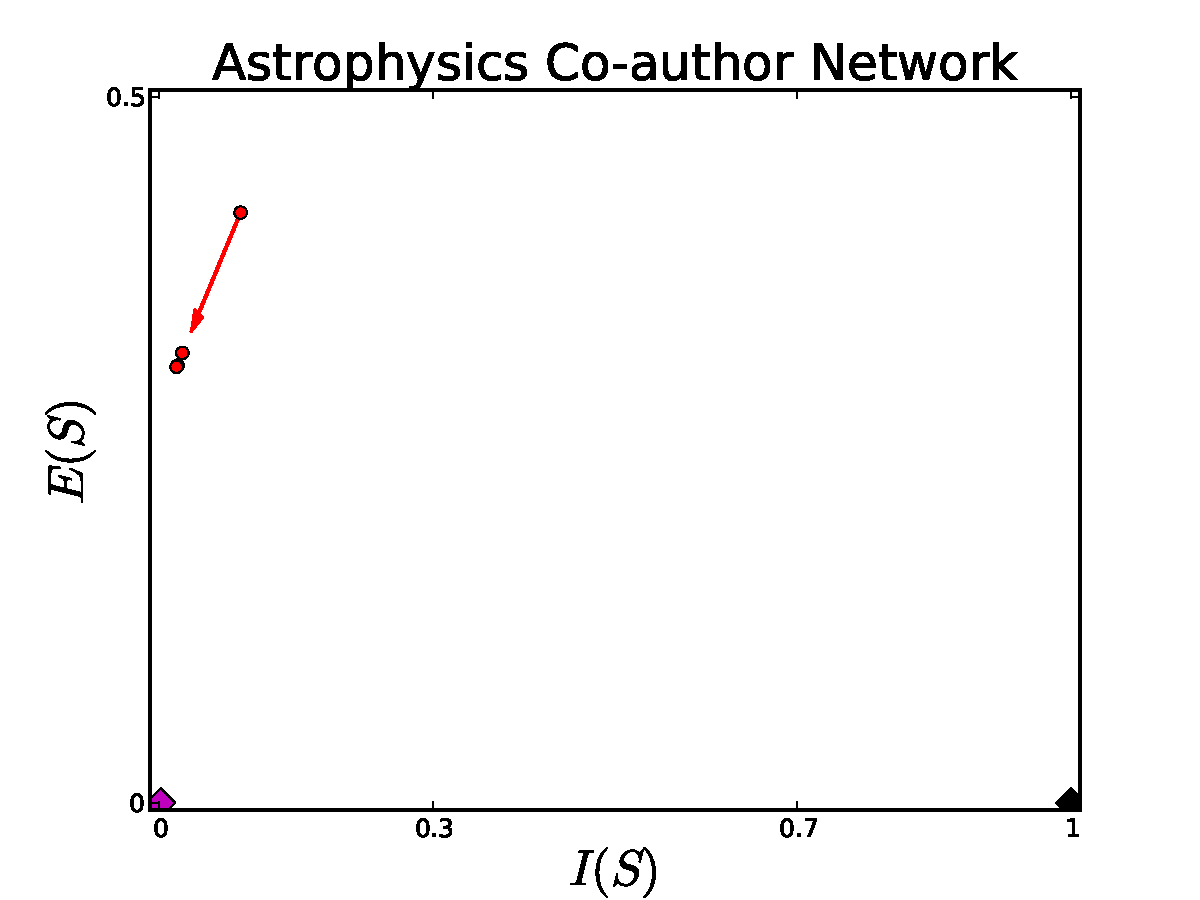
\includegraphics[width=2.8in]{Figures/modularity_astro_sets}
\caption{Here we plot the $(I(S), E(S))$ values produced by each level of the dendogram stages in maximizing modularity with the Louvain algorithm \cite{}.}
\label{fig_real_mod_sets}
\end{figure}


% New Chapter *****************
\chapter{A New Metric: Linearity}

Through our understanding of how existing metrics handle the balance between internal and external density


\section{Single Community Detection}
We maintain that the variables of internal and external density incorporate our full intuition of communities, metrics are just a matter of balancing between the two.  We have shown how previous metrics single communities balance the two or select one to optimize for.  We propose a linear metric that transparently balances between the two variables.
\begin{definition}[Linearity]
 Our metric for single communities:
  \begin{equation}
   \mbox{\sc Linearity} = M_L(C) = a I(C) - b E(C)
  \end{equation}
\end{definition}
Many metrics incorporated the size of the community into their weighting.  Indeed, it is more significant for a large community to gain nearly the same internal density as small community.  Accordingly, there is a generalization of {\sc Linearity} that can account for any desired weighting between internal and external density, with weighting for any size of community.
\begin{definition}[General Metric]
 Our metric for single communities in its greatest generality:
  \begin{equation}
   \mbox{\sc General} = M_G(C)  = \sum\limits_{i = 0} f_i(C) I(C)^i - g_i(C) E(C)^i
  \end{equation}
\end{definition}
Where $f_i$ and $g_i$ can be any function of the size of a community.

Linearity behaves similarly to conductance, when conductance is in a region of the $I,E$ plane where there is a fair balance between improvements of $I$ and $E$.  Unlike conductance though, linearity does not have a critical point in the $I,E$ plane, where the balance is shifted towards only favoring improvements in $E$.  The result is that with the same initial seeds in the Karate Club and CFL, linearity follows the same path as conductance for the first few expansions and stops, rather than engulfing the network.


\subsection{Results}

\begin{theorem}[Single Community Optimization]
If a single metric is optimized and looses $delta_I$, it will not gain it back 
\end{theorem}

\section{Multiple Community Detection}


We now present a linear metric for sets of communities with regard to $I(S)$, $E(S)$, and $|S|$.  It follows the same intuition of creating the linear metric for a single community.  The ideal community is located at $(I(S), E(S), |S|) = (1, 0, 0)$ and accordingly the level sets are parallel planes emanating from around the ideal community.  Hence, the linearity of the metric.  How to balance between improvements in each of the parameters is set by the user.
\begin{definition}[Linearity]
 Our metric for a set of communities:
  \begin{equation}
   \mbox{\sc Linearity}(S) = a I(S) - b E(S) - c |S|,
  \end{equation}
where $a,b,c \geq 0$.
\end{definition}
Depending on the application, communities of certain characteristics may be desired.  Communities of size smaller than a certain size may be desired to be penalized or trade offs between improvements in $E(S)$ and $I(S)$ may depend on existing values.  A general form of this equation is available.
\begin{definition}[General Metric]
 Our metric for single communities in its greatest generality:
  \begin{equation}
   \mbox{\sc General} (S) = \sum\limits_{i = 0} f_i(S) I(S)^i - g_i(S) E(S)^i - h_i |S|^i
  \end{equation}
\end{definition}



\subsection{Results}

\chapter{Parallel Community Detection}

\section {Introduction of Properties and Statistical Significance}

\section{Algorithm}

\subsection{Seeds}

\subsection{Expansion}

\section{Probability of Correctness}

\section {Performance}

\chapter{Case Studies of Networks}

\section{Amazon Product Network}



\section{Collaboration Networks}

\subsection{Astrophysics}

\subsection{Condensed Matter}

\subsection{High Energy Physics}

\subsection{General Relativity}



\section{Enron Email Network}

\section{Epinions Social Network}

\section{Gnutella P2P Network}

\section{Physics Citation Network}

\section{Web Graphs}

\subsection{Berkeley Webpage}

\subsection{Google}


\section{Wiki Network}

\subsection{Communication Network}

\subsection{Election Voting Network}


\chapter{Evolution of Communities}


\chapter{Conclusions}

Above we have provided an indepth look at the details.  Here we provide the summation of our results.

Finding communities is always a tradeoff.  In metric based approaches between internal density and external sparsity.  In significance based approaches the tradeoff is between specificity and sensitivity.

The number of communities a node belongs to follows a power law distribution.

Communities in citation networks evolve from a unioning of previous topics.  However, not all papers that union topics produce successful communities.

\cite{fort}
\cite{porter}
\cite{kanna}
\cite{newman}
\cite{duch}
\cite{blondel}
\cite{mishra}
\cite{jain}
\cite{zhang}
\cite{andersen}
\cite{capocci}
\cite{lanc:2009}
\cite{danon}
\cite{leskovec}
\cite{hui}
\cite{maiya}
\cite{lan:2008}
\cite{hastings}
\cite{leskovec:2008}
\cite{chen}
\cite{lanc:2010}
\cite{girvan}


\appendix
\chapter{Chapter 1 of appendix}
Appendix chapter 1 text goes here

\bibliography{thesis}

\end{document}


\begin{figure}[!h]
\centering
\includegraphics[width=3in]{Figures/ideal_single_community}
\caption{The $(I, E)$ domain for evaluating single communities.  The ideal community is marked by the black square}
\label{fig_ideal_single}
\end{figure}

